% Options for packages loaded elsewhere
\PassOptionsToPackage{unicode}{hyperref}
\PassOptionsToPackage{hyphens}{url}
\PassOptionsToPackage{dvipsnames,svgnames,x11names}{xcolor}
%
\documentclass[
  12pt,
  krantz2]{Format/krantzNoCorner}
\usepackage{amsmath,amssymb}
\usepackage{iftex}
\ifPDFTeX
  \usepackage[T1]{fontenc}
  \usepackage[utf8]{inputenc}
  \usepackage{textcomp} % provide euro and other symbols
\else % if luatex or xetex
  \usepackage{unicode-math} % this also loads fontspec
  \defaultfontfeatures{Scale=MatchLowercase}
  \defaultfontfeatures[\rmfamily]{Ligatures=TeX,Scale=1}
\fi
\usepackage{lmodern}
\ifPDFTeX\else
  % xetex/luatex font selection
\fi
% Use upquote if available, for straight quotes in verbatim environments
\IfFileExists{upquote.sty}{\usepackage{upquote}}{}
\IfFileExists{microtype.sty}{% use microtype if available
  \usepackage[]{microtype}
  \UseMicrotypeSet[protrusion]{basicmath} % disable protrusion for tt fonts
}{}
\makeatletter
\@ifundefined{KOMAClassName}{% if non-KOMA class
  \IfFileExists{parskip.sty}{%
    \usepackage{parskip}
  }{% else
    \setlength{\parindent}{0pt}
    \setlength{\parskip}{6pt plus 2pt minus 1pt}}
}{% if KOMA class
  \KOMAoptions{parskip=half}}
\makeatother
\usepackage{xcolor}
\usepackage{color}
\usepackage{fancyvrb}
\newcommand{\VerbBar}{|}
\newcommand{\VERB}{\Verb[commandchars=\\\{\}]}
\DefineVerbatimEnvironment{Highlighting}{Verbatim}{commandchars=\\\{\}}
% Add ',fontsize=\small' for more characters per line
\usepackage{framed}
\definecolor{shadecolor}{RGB}{248,248,248}
\newenvironment{Shaded}{\begin{snugshade}}{\end{snugshade}}
\newcommand{\AlertTok}[1]{\textcolor[rgb]{0.33,0.33,0.33}{#1}}
\newcommand{\AnnotationTok}[1]{\textcolor[rgb]{0.37,0.37,0.37}{\textbf{\textit{#1}}}}
\newcommand{\AttributeTok}[1]{\textcolor[rgb]{0.27,0.27,0.27}{#1}}
\newcommand{\BaseNTok}[1]{\textcolor[rgb]{0.06,0.06,0.06}{#1}}
\newcommand{\BuiltInTok}[1]{#1}
\newcommand{\CharTok}[1]{\textcolor[rgb]{0.5,0.5,0.5}{#1}}
\newcommand{\CommentTok}[1]{\textcolor[rgb]{0.37,0.37,0.37}{\textit{#1}}}
\newcommand{\CommentVarTok}[1]{\textcolor[rgb]{0.37,0.37,0.37}{\textbf{\textit{#1}}}}
\newcommand{\ConstantTok}[1]{\textcolor[rgb]{0.37,0.37,0.37}{#1}}
\newcommand{\ControlFlowTok}[1]{\textcolor[rgb]{0.27,0.27,0.27}{\textbf{#1}}}
\newcommand{\DataTypeTok}[1]{\textcolor[rgb]{0.27,0.27,0.27}{#1}}
\newcommand{\DecValTok}[1]{\textcolor[rgb]{0.06,0.06,0.06}{#1}}
\newcommand{\DocumentationTok}[1]{\textcolor[rgb]{0.37,0.37,0.37}{\textbf{\textit{#1}}}}
\newcommand{\ErrorTok}[1]{\textcolor[rgb]{0.14,0.14,0.14}{\textbf{#1}}}
\newcommand{\ExtensionTok}[1]{#1}
\newcommand{\FloatTok}[1]{\textcolor[rgb]{0.06,0.06,0.06}{#1}}
\newcommand{\FunctionTok}[1]{\textcolor[rgb]{0.27,0.27,0.27}{\textbf{#1}}}
\newcommand{\ImportTok}[1]{#1}
\newcommand{\InformationTok}[1]{\textcolor[rgb]{0.37,0.37,0.37}{\textbf{\textit{#1}}}}
\newcommand{\KeywordTok}[1]{\textcolor[rgb]{0.27,0.27,0.27}{\textbf{#1}}}
\newcommand{\NormalTok}[1]{#1}
\newcommand{\OperatorTok}[1]{\textcolor[rgb]{0.43,0.43,0.43}{\textbf{#1}}}
\newcommand{\OtherTok}[1]{\textcolor[rgb]{0.37,0.37,0.37}{#1}}
\newcommand{\PreprocessorTok}[1]{\textcolor[rgb]{0.37,0.37,0.37}{\textit{#1}}}
\newcommand{\RegionMarkerTok}[1]{#1}
\newcommand{\SpecialCharTok}[1]{\textcolor[rgb]{0.43,0.43,0.43}{\textbf{#1}}}
\newcommand{\SpecialStringTok}[1]{\textcolor[rgb]{0.5,0.5,0.5}{#1}}
\newcommand{\StringTok}[1]{\textcolor[rgb]{0.5,0.5,0.5}{#1}}
\newcommand{\VariableTok}[1]{\textcolor[rgb]{0,0,0}{#1}}
\newcommand{\VerbatimStringTok}[1]{\textcolor[rgb]{0.5,0.5,0.5}{#1}}
\newcommand{\WarningTok}[1]{\textcolor[rgb]{0.37,0.37,0.37}{\textbf{\textit{#1}}}}
\usepackage{longtable,booktabs,array}
\usepackage{calc} % for calculating minipage widths
% Correct order of tables after \paragraph or \subparagraph
\usepackage{etoolbox}
\makeatletter
\patchcmd\longtable{\par}{\if@noskipsec\mbox{}\fi\par}{}{}
\makeatother
% Allow footnotes in longtable head/foot
\IfFileExists{footnotehyper.sty}{\usepackage{footnotehyper}}{\usepackage{footnote}}
\makesavenoteenv{longtable}
\usepackage{graphicx}
\makeatletter
\def\maxwidth{\ifdim\Gin@nat@width>\linewidth\linewidth\else\Gin@nat@width\fi}
\def\maxheight{\ifdim\Gin@nat@height>\textheight\textheight\else\Gin@nat@height\fi}
\makeatother
% Scale images if necessary, so that they will not overflow the page
% margins by default, and it is still possible to overwrite the defaults
% using explicit options in \includegraphics[width, height, ...]{}
\setkeys{Gin}{width=\maxwidth,height=\maxheight,keepaspectratio}
% Set default figure placement to htbp
\makeatletter
\def\fps@figure{htbp}
\makeatother
\setlength{\emergencystretch}{3em} % prevent overfull lines
\providecommand{\tightlist}{%
  \setlength{\itemsep}{0pt}\setlength{\parskip}{0pt}}
\setcounter{secnumdepth}{5}

\usepackage{booktabs}
\usepackage{empheq}
\setcounter{secnumdepth}{2}

\usepackage{amsfonts}
\usepackage{amsmath}
\usepackage{amssymb}
\usepackage{array}
\usepackage{caption}
\captionsetup[figureNoLabel]{labelformat=empty, justification=raggedright}

\usepackage{color}
\usepackage{colortbl}
\usepackage{xcolor}
\usepackage{xr}


\usepackage{fancyvrb}
\usepackage{framed}
\setlength{\fboxsep}{.8em}

\usepackage{graphicx}

\usepackage{multirow}
\usepackage{tabularx}

\usepackage{setspace}
\usepackage{scalefnt}

\usepackage{verbatim}

\usepackage{mdframed}

\definecolor{lightgray}{gray}{0.98}

% Custom environment for background box
\newmdenv[
  backgroundcolor=lightgray,
  skipabove=10pt,
  skipbelow=10pt,
  leftmargin=0,
  rightmargin=0,
  innerleftmargin=10pt,
  innerrightmargin=10pt,
  innertopmargin=10pt,
  innerbottommargin=10pt
]{graybox}

\newenvironment{blackbox}{
  \definecolor{shadecolor}{rgb}{0, 0, 0}  % black
  \color{white}
  \begin{shaded}}
 {\end{shaded}}
 
% \newenvironment{greybox}{
%   \definecolor{shadecolor}{rgb}{0.9, 0.9, 0.9}  % light grey??
%   \color{white}
%   \begin{shaded}}
%  {\end{shaded}}
 
% \usepackage[left=1in,top=1in,right=1in,bottom=1in]{geometry}



%\usepackage{wrapfig}



\setlength{\fboxsep}{.8em}

\renewcommand{\hrulefill}{%
  \leavevmode\leaders\hrule height 2pt\hfill\kern0pt }
  
\renewcommand{\dotfill}{%
  \leavevmode\cleaders\hbox to 0.60em{\hss .\hss }\hfill\kern0pt }

\usepackage{makeidx}
\makeindex

\usepackage{booktabs}
\usepackage{longtable}
\usepackage{array}
\usepackage{multirow}
\usepackage{wrapfig}
\usepackage{float}
\usepackage{colortbl}
\usepackage{pdflscape}
\usepackage{tabu}
\usepackage{threeparttable}
\usepackage{threeparttablex}
\usepackage[normalem]{ulem}
\usepackage{makecell}
\usepackage{xcolor}
\ifLuaTeX
  \usepackage{selnolig}  % disable illegal ligatures
\fi
\usepackage[]{natbib}
\bibliographystyle{Format/econPeriod}
\IfFileExists{bookmark.sty}{\usepackage{bookmark}}{\usepackage{hyperref}}
\IfFileExists{xurl.sty}{\usepackage{xurl}}{} % add URL line breaks if available
\urlstyle{same}
\hypersetup{
  pdftitle={Loss Data Analytics   Second Edition},
  pdfauthor={An open text authored by the Actuarial Community},
  colorlinks=true,
  linkcolor={Maroon},
  filecolor={Maroon},
  citecolor={Blue},
  urlcolor={Blue},
  pdfcreator={LaTeX via pandoc}}

\title{Loss Data Analytics \newline Second Edition}
\author{An open text authored by the Actuarial Community}
\date{}

\begin{document}
\maketitle

{
\hypersetup{linkcolor=}
\setcounter{tocdepth}{2}
\tableofcontents
}
\hypertarget{preface}{%
\chapter*{Preface}\label{preface}}


\emph{Date: 19 September 2024}

\hypertarget{book-description}{%
\subsubsection*{Book Description}\label{book-description}}


\textbf{Loss Data Analytics} is an interactive, online, freely available text.

\begin{itemize}
\tightlist
\item
  The online version contains many interactive objects (quizzes, computer demonstrations, interactive graphs, video, and the like) to promote \emph{deeper learning}.
\item
  A subset of the book is available for \emph{offline reading} in pdf and EPUB formats.
\item
  The online text will be available in multiple languages to promote access to a \emph{worldwide audience}.
\end{itemize}

\hypertarget{what-will-success-look-like}{%
\subsubsection*{What will success look like?}\label{what-will-success-look-like}}


The online text will be freely available to a worldwide audience. The online version will contain many interactive objects (quizzes, computer demonstrations, interactive graphs, video, and the like) to promote deeper learning. Moreover, a subset of the book will be available in pdf format for low-cost printing. The online text will be available in multiple languages to promote access to a worldwide audience.

\hypertarget{how-will-the-text-be-used}{%
\subsubsection*{How will the text be used?}\label{how-will-the-text-be-used}}


This book will be useful in actuarial curricula worldwide. It will cover the loss data learning objectives of the major actuarial organizations. Thus, it will be suitable for classroom use at universities as well as for use by independent learners seeking to pass professional actuarial examinations. Moreover, the text will also be useful for the continuing professional development of actuaries and other professionals in insurance and related financial risk management industries.

\hypertarget{why-is-this-good-for-the-profession}{%
\subsubsection*{Why is this good for the profession?}\label{why-is-this-good-for-the-profession}}


An online text is a type of open educational resource (OER). One important benefit of an OER is that it equalizes access to knowledge, thus permitting a broader community to learn about the actuarial profession. Moreover, it has the capacity to engage viewers through active learning that deepens the learning process, producing analysts more capable of solid actuarial work.

Why is this good for students and teachers and others involved in the learning process? Cost is often cited as an important factor for students and teachers in textbook selection (see a recent post on the \href{https://www.aei.org/publication/the-new-era-of-the-400-college-textbook-which-is-part-of-the-unsustainable-higher-education-bubble/}{\$400 textbook}). Students will also appreciate the ability to ``carry the book around'' on their mobile devices.

\hypertarget{why-loss-data-analytics}{%
\subsubsection*{Why loss data analytics?}\label{why-loss-data-analytics}}


The intent is that this type of resource will eventually permeate throughout the actuarial curriculum. Given the dramatic changes in the way that actuaries treat data, loss data seems like a natural place to start. The idea behind the name \emph{loss data analytics} is to integrate classical loss data models from applied probability with modern analytic tools. In particular, we recognize that big data (including social media and usage based insurance) are here to stay and that high speed computation is readily available.

\hypertarget{project-goal}{%
\subsubsection*{Project Goal}\label{project-goal}}


The project goal is to have the actuarial community author our textbooks in a collaborative fashion. To get involved, please visit our
\href{https://sites.google.com/a/wisc.edu/loss-data-analytics/}{Open Actuarial Textbooks Project Site}.

\hypertarget{acknowledgements}{%
\section*{Acknowledgements}\label{acknowledgements}}


Edward Frees acknowledges the John and Anne Oros Distinguished Chair for Inspired Learning in Business which provided seed money to support the project. Frees and his Wisconsin colleagues also acknowledge a Society of Actuaries Center of Excellence Grant that provided funding to support work in dependence modeling and health initiatives. Wisconsin also provided an education innovation grant that provided partial support for the many students who have worked on this project.

We acknowledge the Society of Actuaries for permission to use problems from their examinations.

We thank Rob Hyndman, Monash University, for allowing us to use his excellent style files to produce the online version of the book.

We thank Yihui Xie and his colleagues at \href{https://www.rstudio.com/}{Rstudio} for the \href{https://bookdown.org/yihui/bookdown/}{R bookdown} package that allows us to produce this book.

We also wish to acknowledge the support and sponsorship of the \href{http://www.blackactuaries.org/}{International Association of Black Actuaries} in our joint efforts to provide actuarial educational content to all.


\includegraphics[width=0.25\textwidth,height=\textheight]{Figures/IABA.png}

\hypertarget{contributors}{%
\section*{Contributors}\label{contributors}}


The project goal is to have the actuarial community author our textbooks in a collaborative fashion. The following contributors have taken a leadership role in developing \emph{Loss Data Analytics}.

\begin{center}\rule{0.5\linewidth}{0.5pt}\end{center}

\begin{center}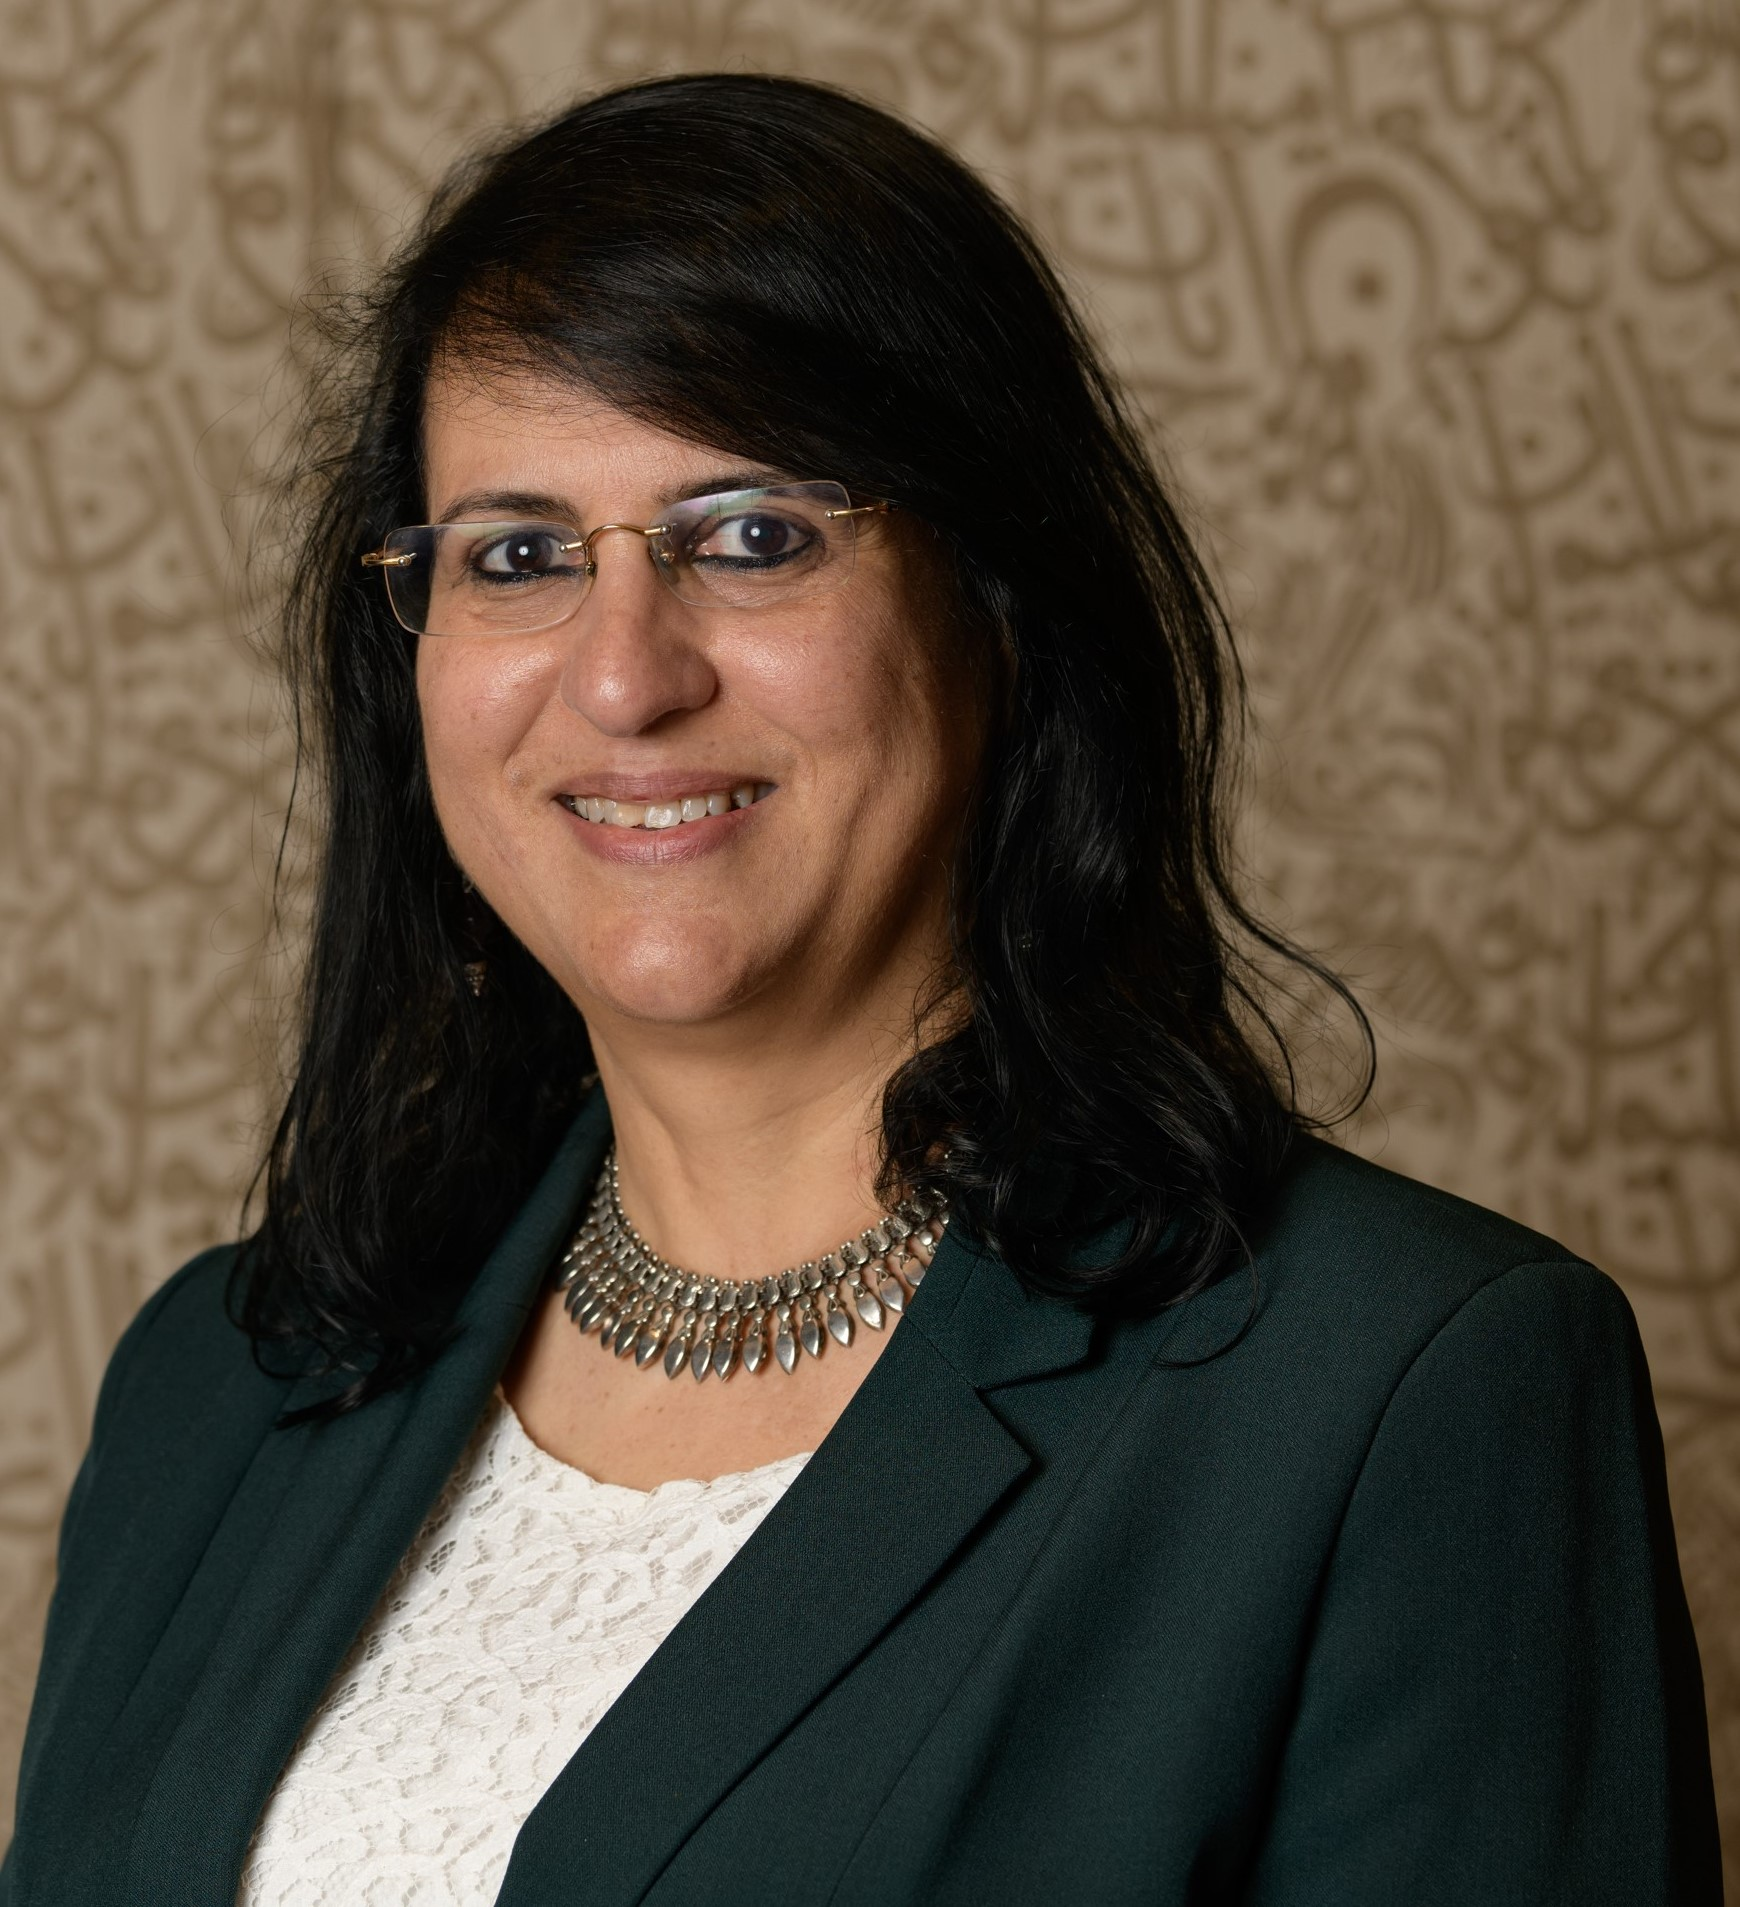
\includegraphics[width=0.2\linewidth,height=0.3\textheight]{ContributorPics/ZeinabAmin} \end{center}

\begin{center}
\textbf{ Zeinab Amin }
\end{center}

\begin{itemize}
\item
  \textbf{Zeinab Amin} is a Professor at the Department of Mathematics and Actuarial Science and Associate Provost for Assessment and Accreditation at the American University in Cairo (AUC). Amin holds a PhD in Statistics and is an Associate of the Society of Actuaries. Amin is the recipient of the 2016 Excellence in Academic Service Award and the 2009 Excellence in Teaching Award from AUC. Amin has designed and taught a variety of statistics and actuarial science courses. Amin's current area of research includes quantitative risk assessment, reliability assessment, general statistical modelling, and Bayesian statistics.
\item
  \textbf{Katrien Antonio}, KU Leuven
\end{itemize}

\begin{center}\rule{0.5\linewidth}{0.5pt}\end{center}

\newpage

\begin{center}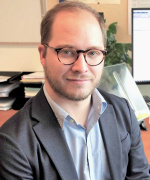
\includegraphics[width=0.2\linewidth,height=0.3\textheight]{ContributorPics/JFBegin} \end{center}

\begin{center}
\textbf{ Jean-François Bégin }
\end{center}

\begin{itemize}
\item
  \textbf{Jean-François Bégin} is an Assistant Professor in the Department of Statistics and Actuarial Science at Simon Fraser University in British Columbia, Canada. Bégin holds a PhD in Financial Engineering from HEC Montréal, Canada, and is a Fellow of the Society of Actuaries and of the Canadian Institute of Actuaries. His current research interests include financial modelling, financial econometrics, Bayesian statistics, filtering methods, credit risk, option pricing, and pension economics. Bégin has designed and taught a variety of actuarial finance and actuarial communication courses.
\item
  \textbf{Jan Beirlant}, KU Leuven
\end{itemize}

\begin{center}\rule{0.5\linewidth}{0.5pt}\end{center}

\begin{center}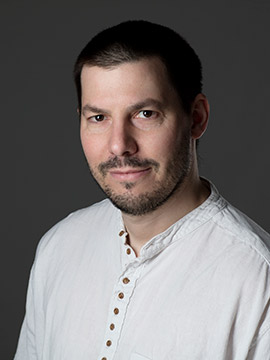
\includegraphics[width=0.2\linewidth,height=0.3\textheight]{ContributorPics/Charpentier} \end{center}

\begin{center}
\textbf{ Arthur Charpentier }
\end{center}

\begin{itemize}
\tightlist
\item
  \textbf{Arthur Charpentier} is a professor in the Department of Mathematics at the Université du Québec á Montréal.~Prior to that, he worked at a large general insurance company in Hong Kong, China, and the French Federation of Insurers in Paris, France. He received a MS on mathematical economics at Université Paris Dauphine and a MS in actuarial science at ENSAE (National School of Statistics) in Paris, and a PhD degree from KU Leuven, Belgium. His research interests include econometrics, applied probability and actuarial science. He has published several books (the most recent one on \emph{Computational Actuarial Science with R}, CRC) and papers on a variety of topics. He is a Fellow of the French Institute of Actuaries, and was in charge of the `Data Science for Actuaries' program from 2015 to 2018.
\end{itemize}

\begin{center}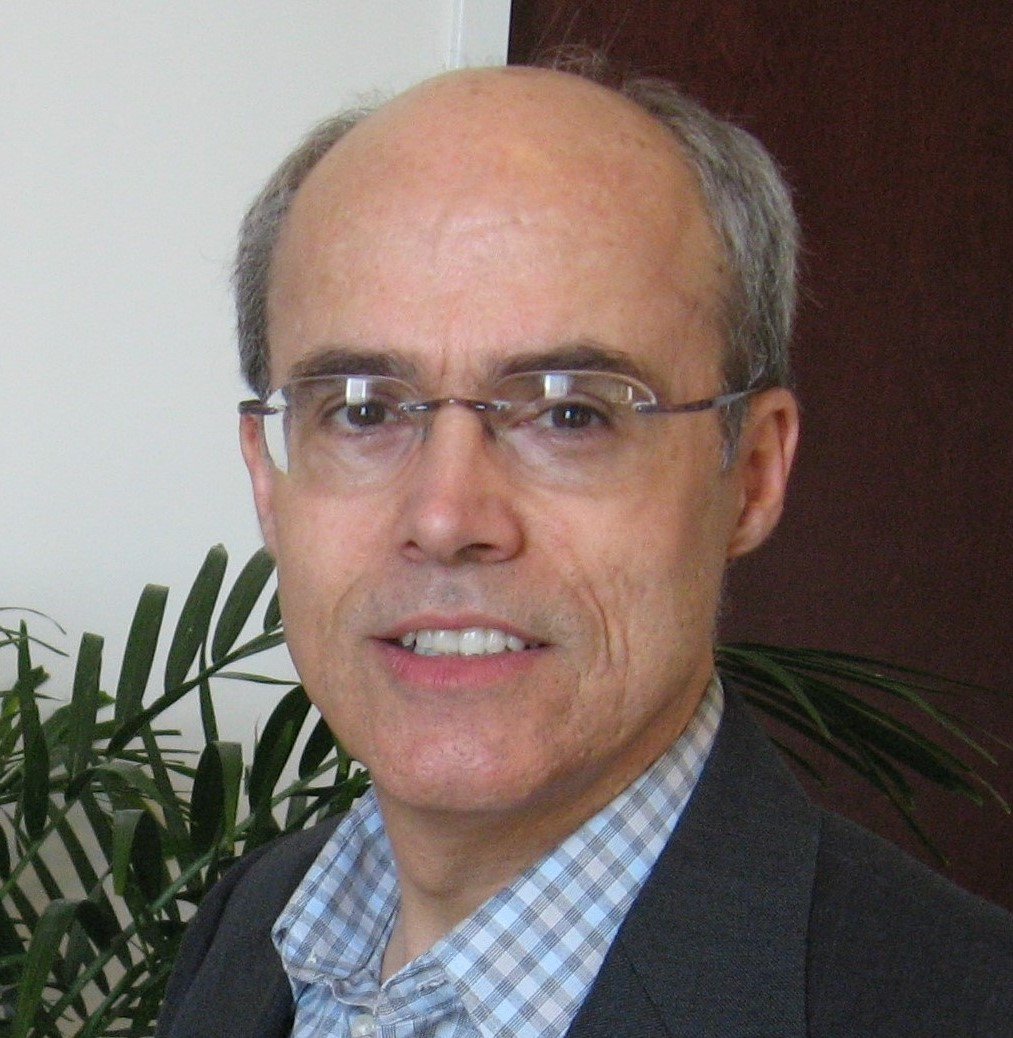
\includegraphics[width=0.2\linewidth,height=0.3\textheight]{ContributorPics/PhotoGaryDean} \end{center}

\begin{center}
\textbf{ Curtis Gary Dean }
\end{center}

\begin{itemize}
\tightlist
\item
  \textbf{Curtis Gary Dean} is the Lincoln Financial Distinguished Professor of Actuarial Science at Ball State University. He is a Fellow of the Casualty Actuarial Society and a CFA charterholder. He has extensive practical experience as an actuary at American States Insurance, SAFECO, and Travelers. He has served the CAS and actuarial profession as chair of the Examination Committee, first editor-in-chief for \emph{Variance: Advancing the Science of Risk}, and as a member of the Board of Directors and the Executive Council. He contributed a chapter to \emph{Predictive Modeling Applications in Actuarial Science} published by Cambridge University Press.
\end{itemize}

\begin{center}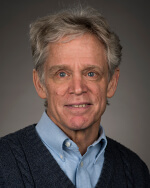
\includegraphics[width=0.2\linewidth,height=0.3\textheight]{ContributorPics/Frees_Jed2018_150x188} \end{center}

\begin{center}
\textbf{ Edward (Jed) Frees }
\end{center}

\begin{itemize}
\tightlist
\item
  \textbf{Edward (Jed) Frees} is an emeritus professor, formerly the Hickman-Larson Chair of Actuarial Science at the University of Wisconsin-Madison. He is a Fellow of both the Society of Actuaries and the American Statistical Association. He has published extensively (a four-time winner of the Halmstad and Prize for best paper published in the actuarial literature) and has written three books. He also is a co-editor of the two-volume series \emph{Predictive Modeling Applications in Actuarial Science} published by Cambridge University Press.
\end{itemize}

\newpage

\begin{center}
\includegraphics[width=0.2\linewidth,height=0.3\textheight]{ContributorPics/GuojunGan} \end{center}

\begin{center}
\textbf{ Guojun Gan }
\end{center}

\begin{itemize}
\tightlist
\item
  \textbf{Guojun Gan} is an associate professor in the Department of Mathematics at the University of Connecticut, where he has been since August 2014. Prior to that, he worked at a large life insurance company in Toronto, Canada for six years. He received a BS degree from Jilin University, Changchun, China, in 2001 and MS and PhD degrees from York University, Toronto, Canada, in 2003 and 2007, respectively. His research interests include data mining and actuarial science. He has published several books and papers on a variety of topics, including data clustering, variable annuity, mathematical finance, applied statistics, and VBA programming.
\end{itemize}

\begin{center}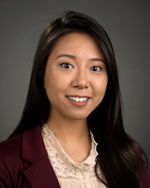
\includegraphics[width=0.2\linewidth,height=0.3\textheight]{ContributorPics/Gao_Lisa_150x188} \end{center}

\begin{center}
\textbf{ Lisa Gao }
\end{center}

\begin{itemize}
\tightlist
\item
  \textbf{Lisa Gao} is a PhD candidate in the Risk and Insurance department at the University of Wisconsin-Madison. She holds a BMath in Actuarial Science and Statistics from the University of Waterloo and is an Associate of the Society of Actuaries.
\end{itemize}

\begin{itemize}
\tightlist
\item
  \textbf{José Garrido}, Concordia University
\end{itemize}

\begin{center}\rule{0.5\linewidth}{0.5pt}\end{center}

\begin{center}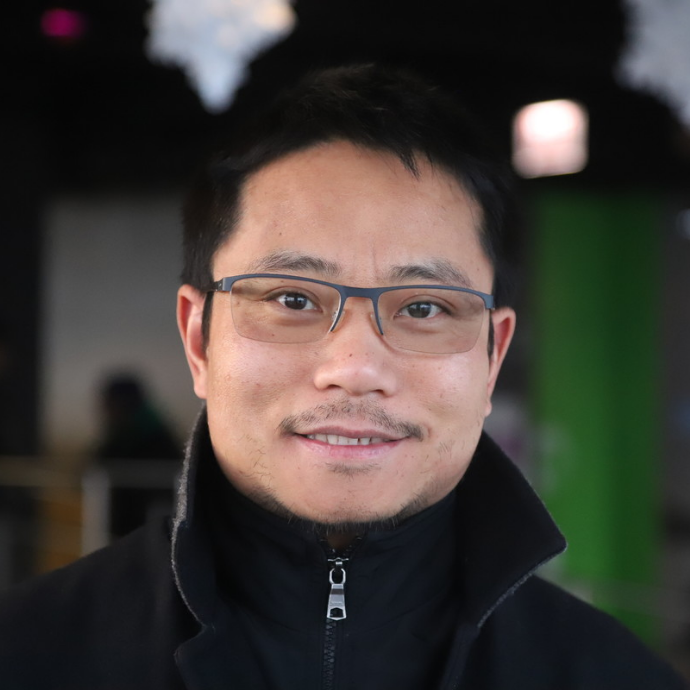
\includegraphics[width=0.2\linewidth,height=0.3\textheight]{ContributorPics/Larry2018} \end{center}

\begin{center}
\textbf{ Lei (Larry) Hua }
\end{center}

\begin{itemize}
\tightlist
\item
  \textbf{Lei (Larry) Hua} is an Associate Professor of Actuarial Science at Northern Illinois University. He earned a PhD degree in Statistics from the University of British Columbia. He is an Associate of the Society of Actuaries. His research work focuses on multivariate dependence modeling for non-Gaussian phenomena and innovative applications for financial and insurance industries.
\end{itemize}

\begin{center}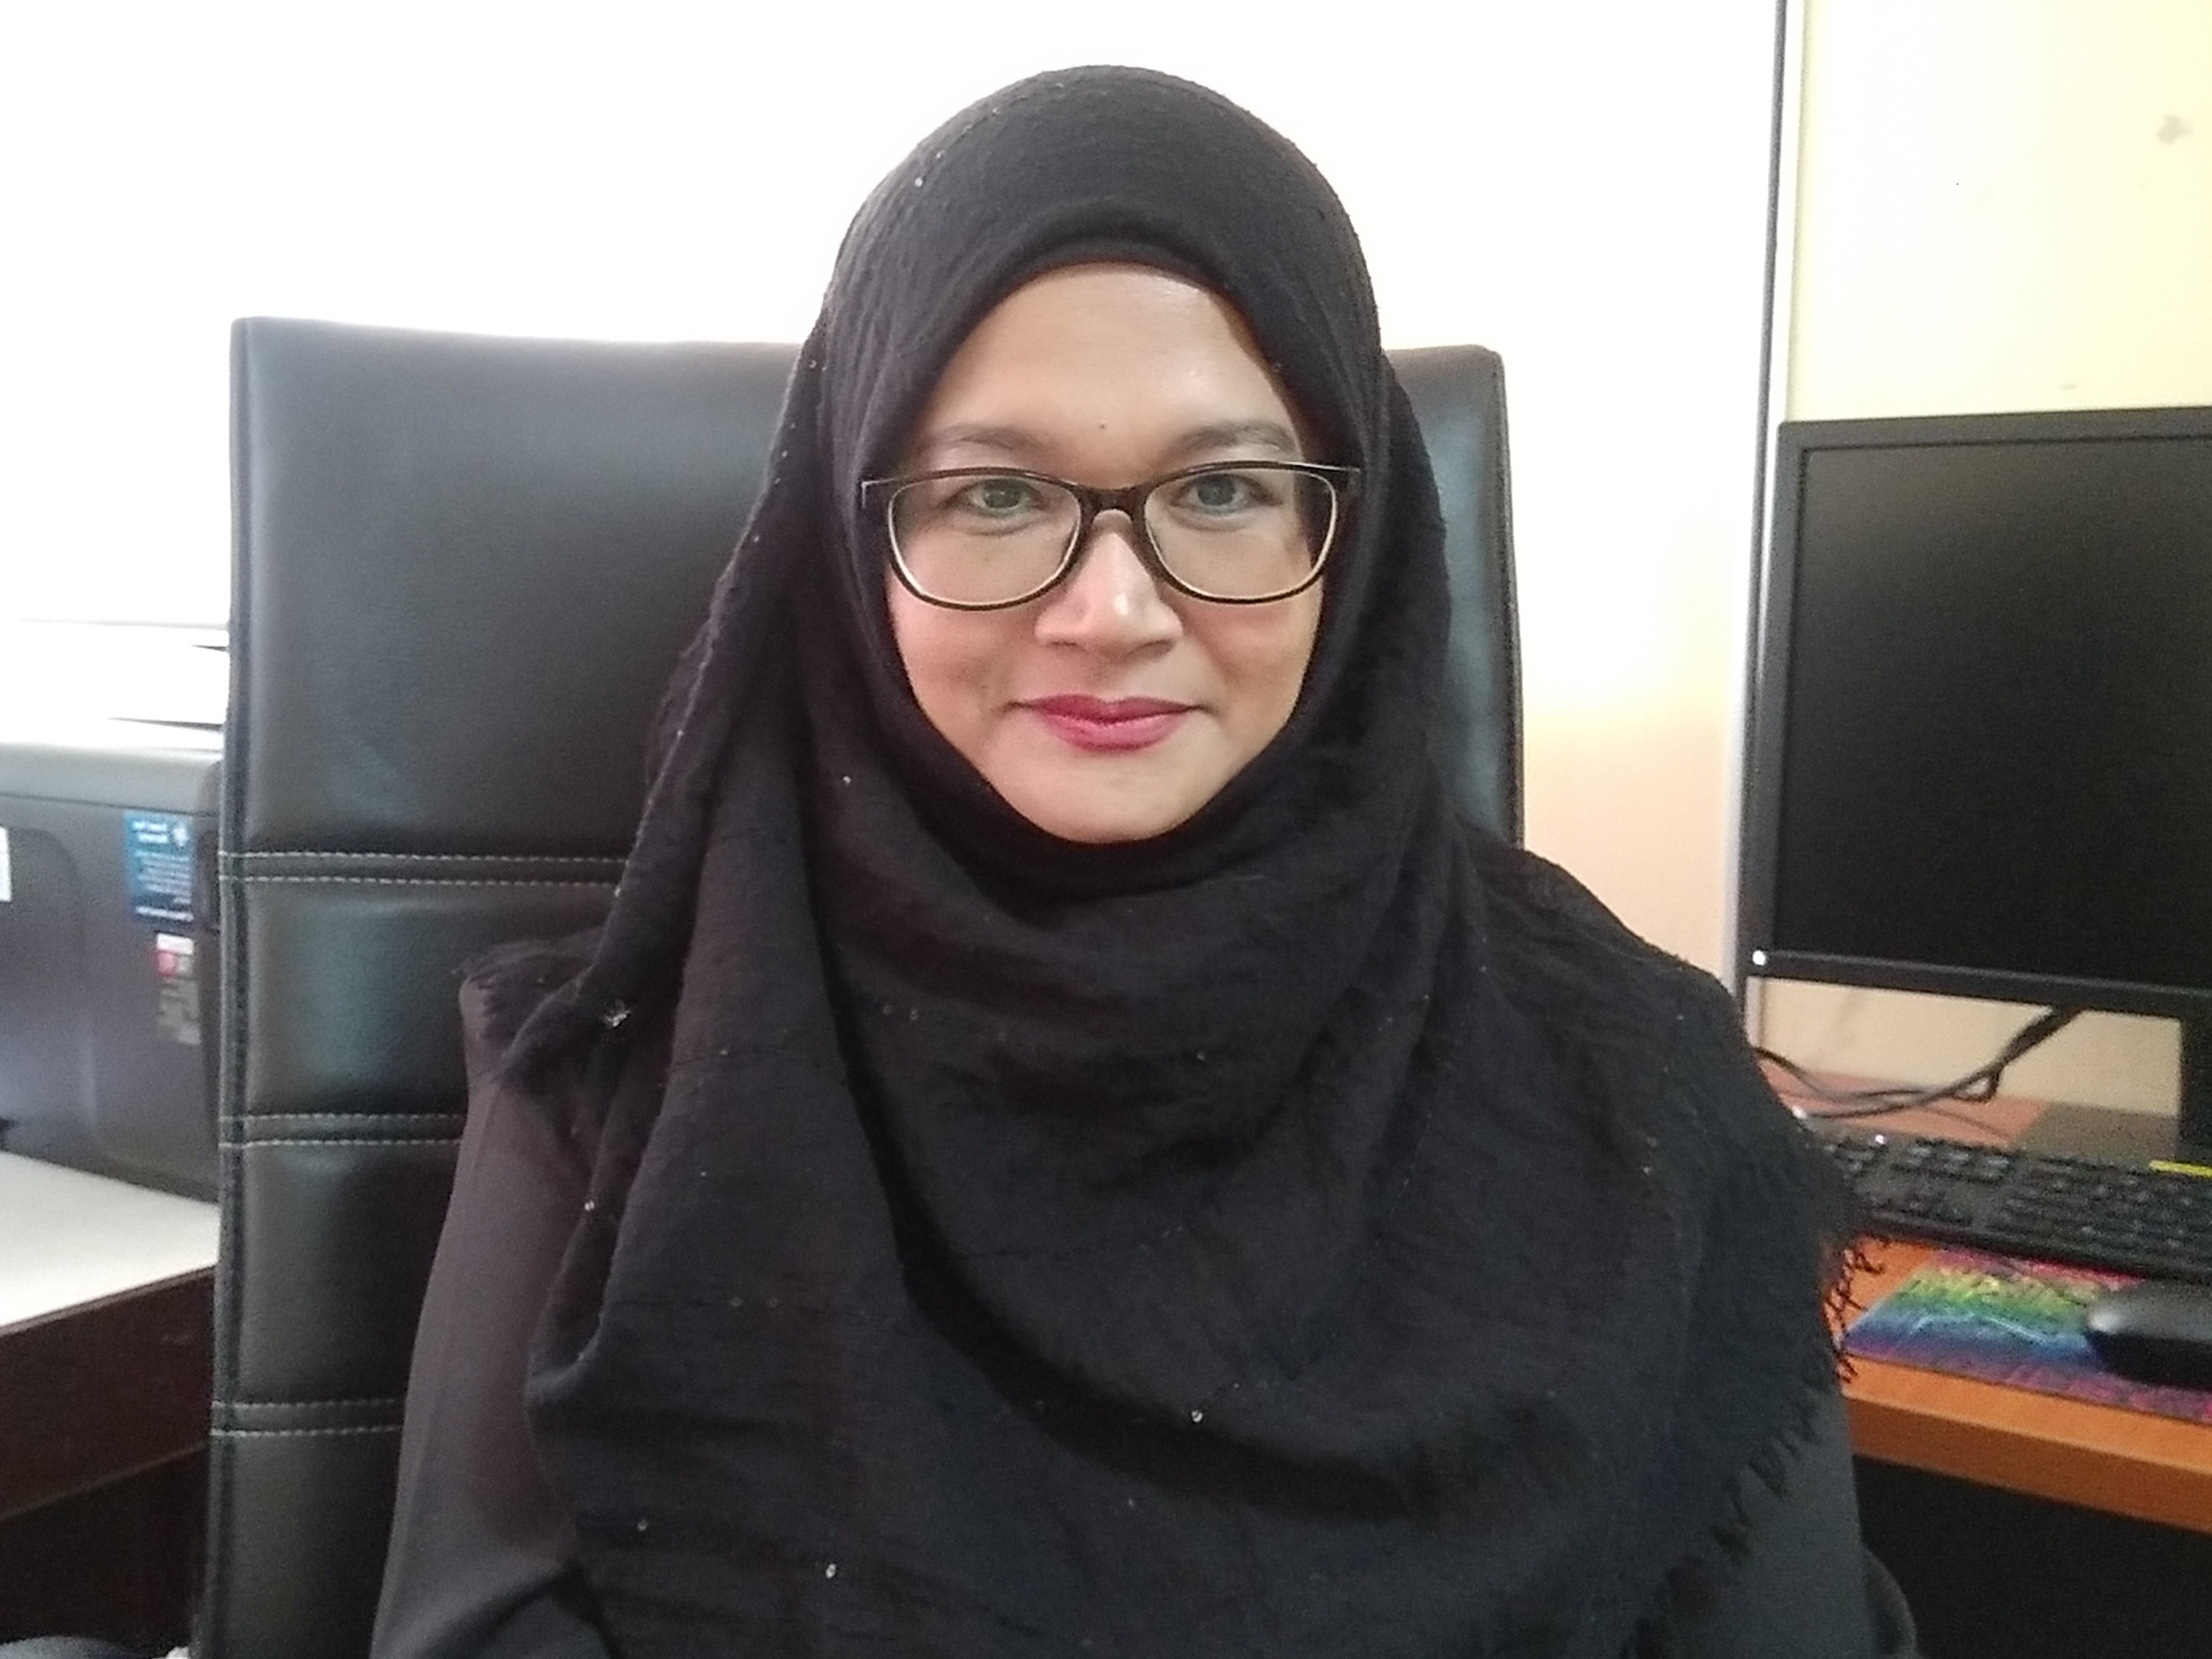
\includegraphics[width=0.2\linewidth,height=0.3\textheight]{ContributorPics/Noriszura} \end{center}

\begin{center}
\textbf{ Noriszura Ismail }
\end{center}

\begin{itemize}
\tightlist
\item
  \textbf{Noriszura Ismail} is a Professor and Head of Actuarial Science Program, Universiti Kebangsaan Malaysia (UKM). She specializes in Risk Modelling and Applied Statistics. She obtained her BSc and MSc (Actuarial Science) in 1991 and 1993 from University of Iowa, and her PhD (Statistics) in 2007 from UKM. She also passed several papers from Society of Actuaries in 1994. She has received several research grants from Ministry of Higher Education Malaysia (MOHE) and UKM, totaling about MYR1.8 million. She has successfully supervised and co-supervised several PhD students (13 completed and 11 on-going). She currently has about 180 publications, consisting of 88 journals and 95 proceedings.
\end{itemize}

\begin{center}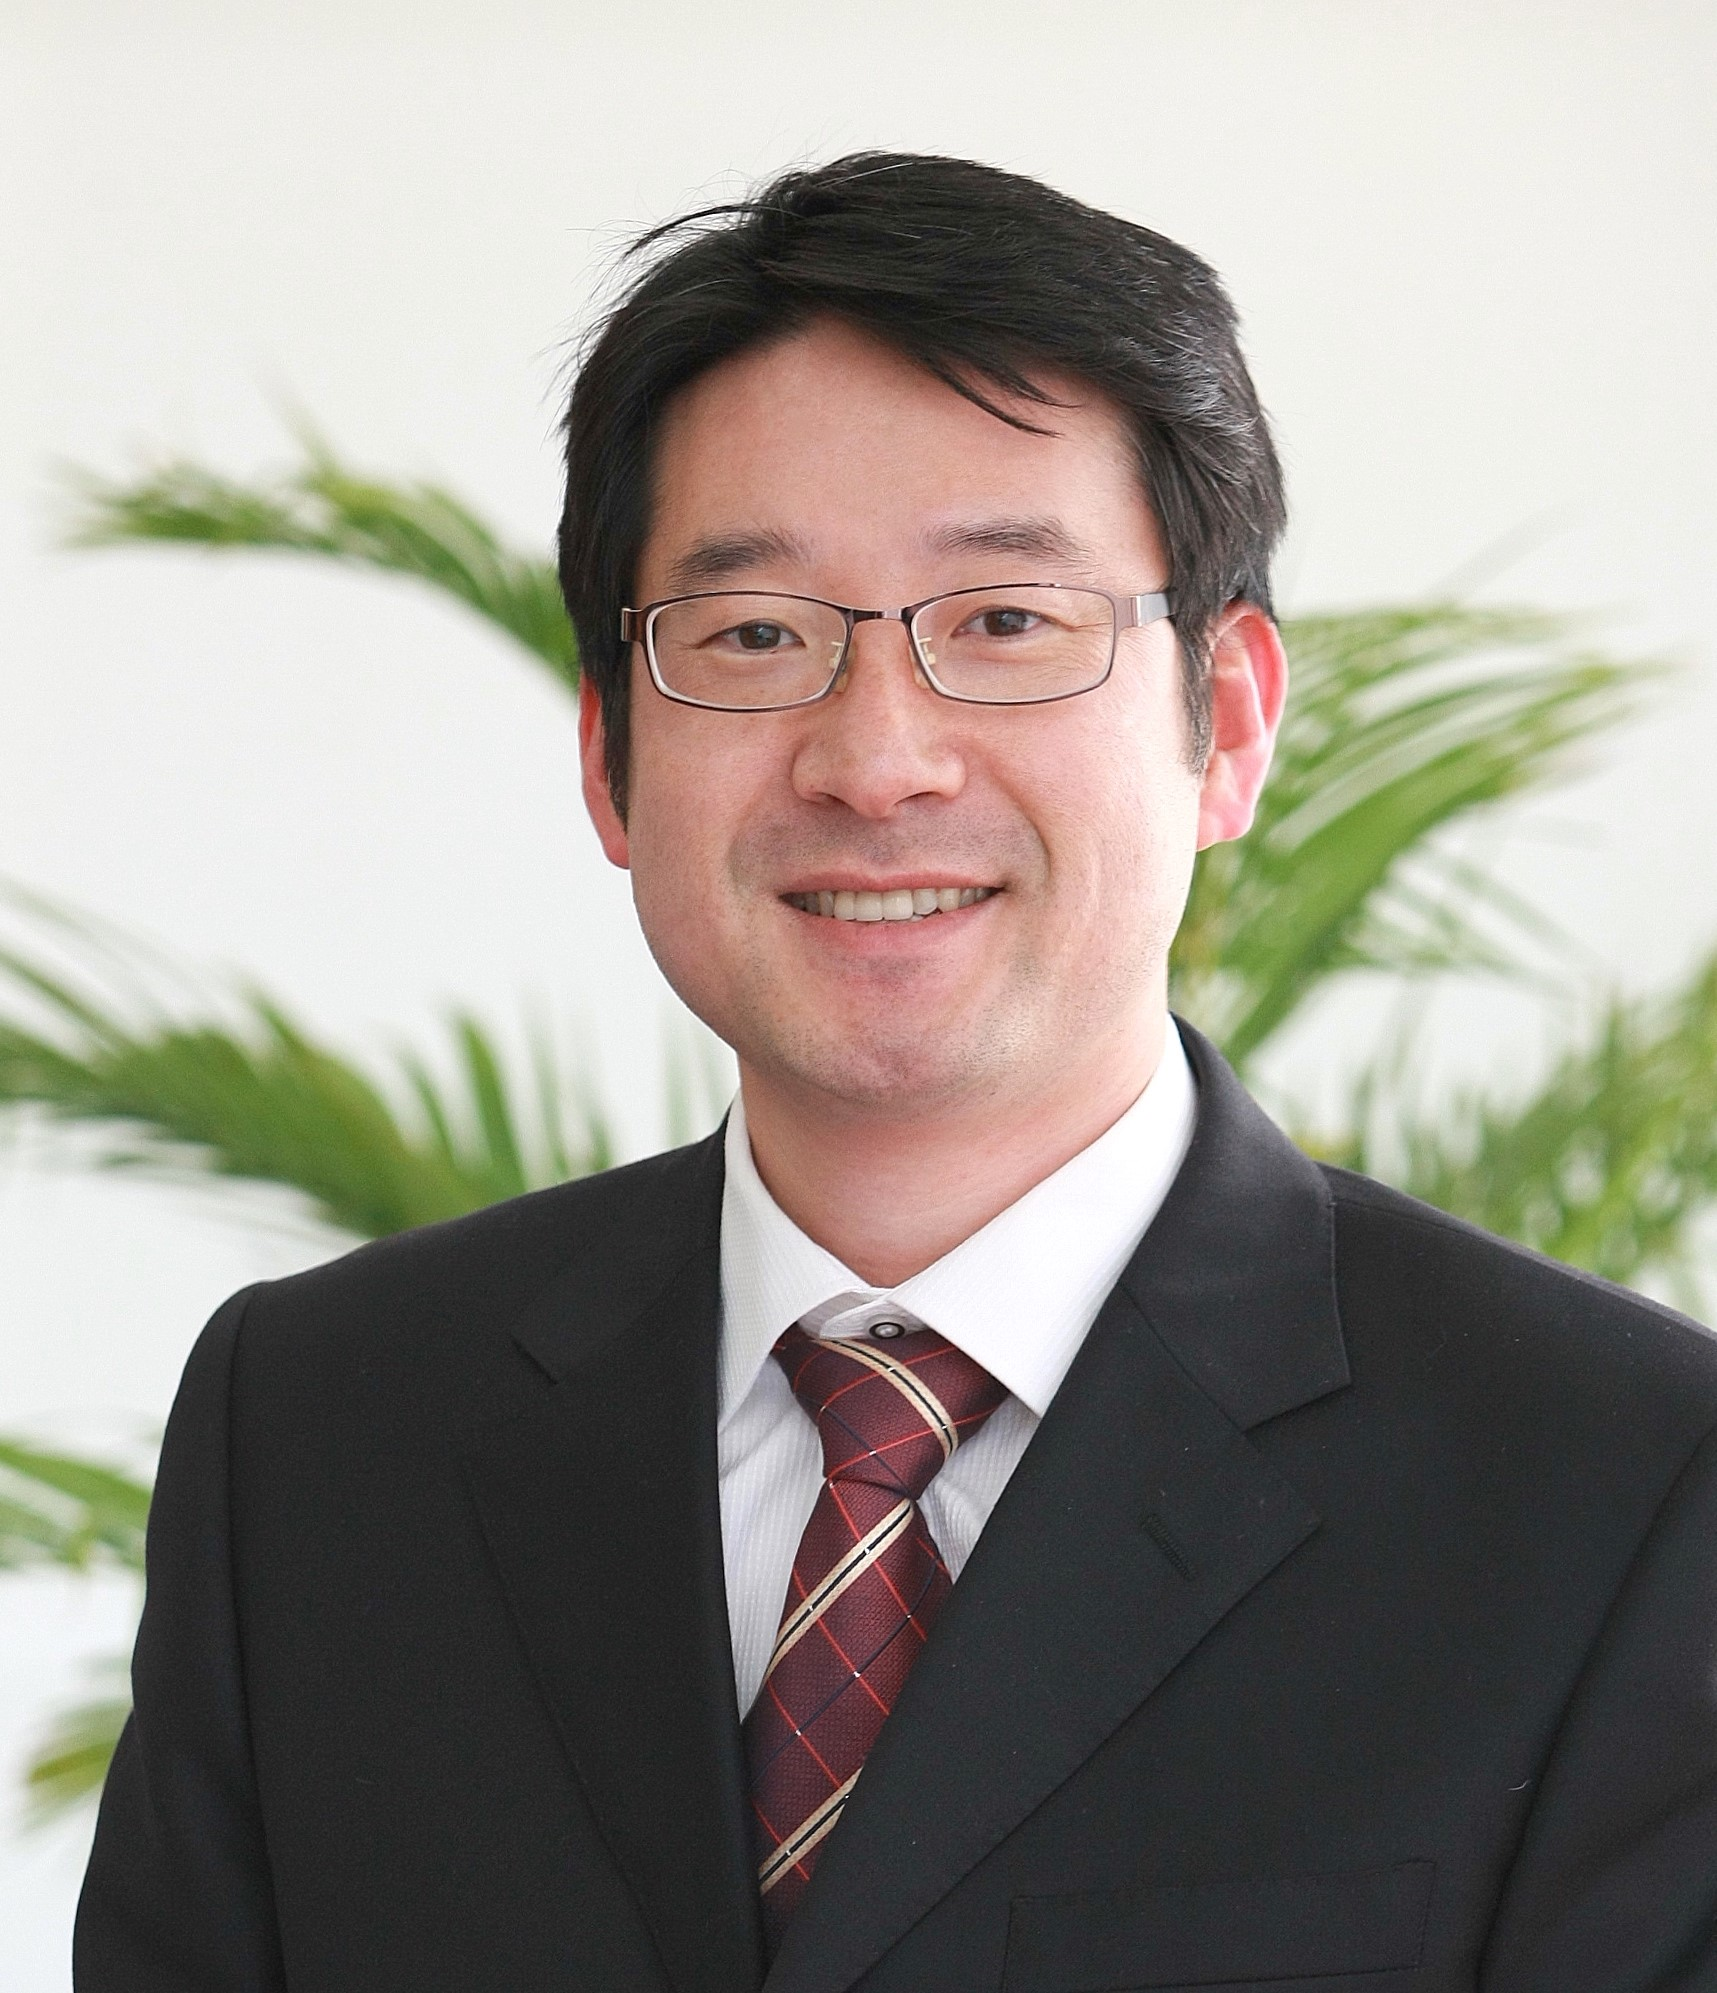
\includegraphics[width=0.2\linewidth,height=0.3\textheight]{ContributorPics/JosephKimPic} \end{center}

\begin{center}
\textbf{ Joseph H.T. Kim }
\end{center}

\begin{itemize}
\tightlist
\item
  \textbf{Joseph H.T. Kim}, Ph.D., FSA, CERA, is Associate Professor of Applied Statistics at Yonsei University, Seoul, Korea. He holds a Ph.D.~degree in Actuarial Science from the University of Waterloo, at which he taught as Assistant Professor. He also worked in the life insurance industry. He has published papers in \emph{Insurance Mathematics and Economics}, \emph{Journal of Risk and Insurance}, \emph{Journal of Banking and Finance}, \emph{ASTIN Bulletin}, and \emph{North American Actuarial Journal}, among others.
\end{itemize}

\begin{center}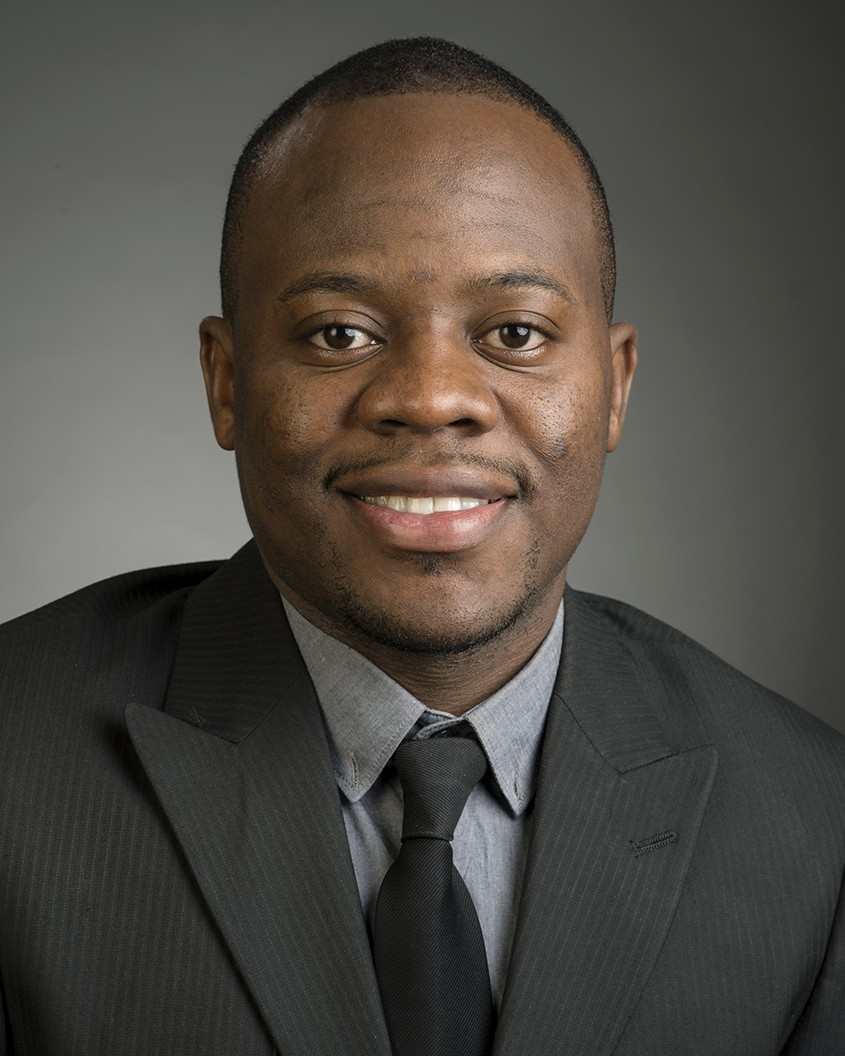
\includegraphics[width=0.2\linewidth,height=0.3\textheight]{ContributorPics/Okine_A} \end{center}

\begin{center}
\textbf{ Nii-Armah Okine }
\end{center}

\begin{itemize}
\tightlist
\item
  \textbf{Nii-Armah Okine} is an assistant professor at the Mathematical Sciences Department at Appalachian State University. He holds a Ph.D.~in Business (Actuarial Science) from the University of Wisconsin - Madison and obtained his master's degree in Actuarial science from Illinois State University. His research interest includes micro-level reserving, joint longitudinal-survival modeling, dependence modeling, micro-insurance, and machine learning.
\end{itemize}

\begin{center}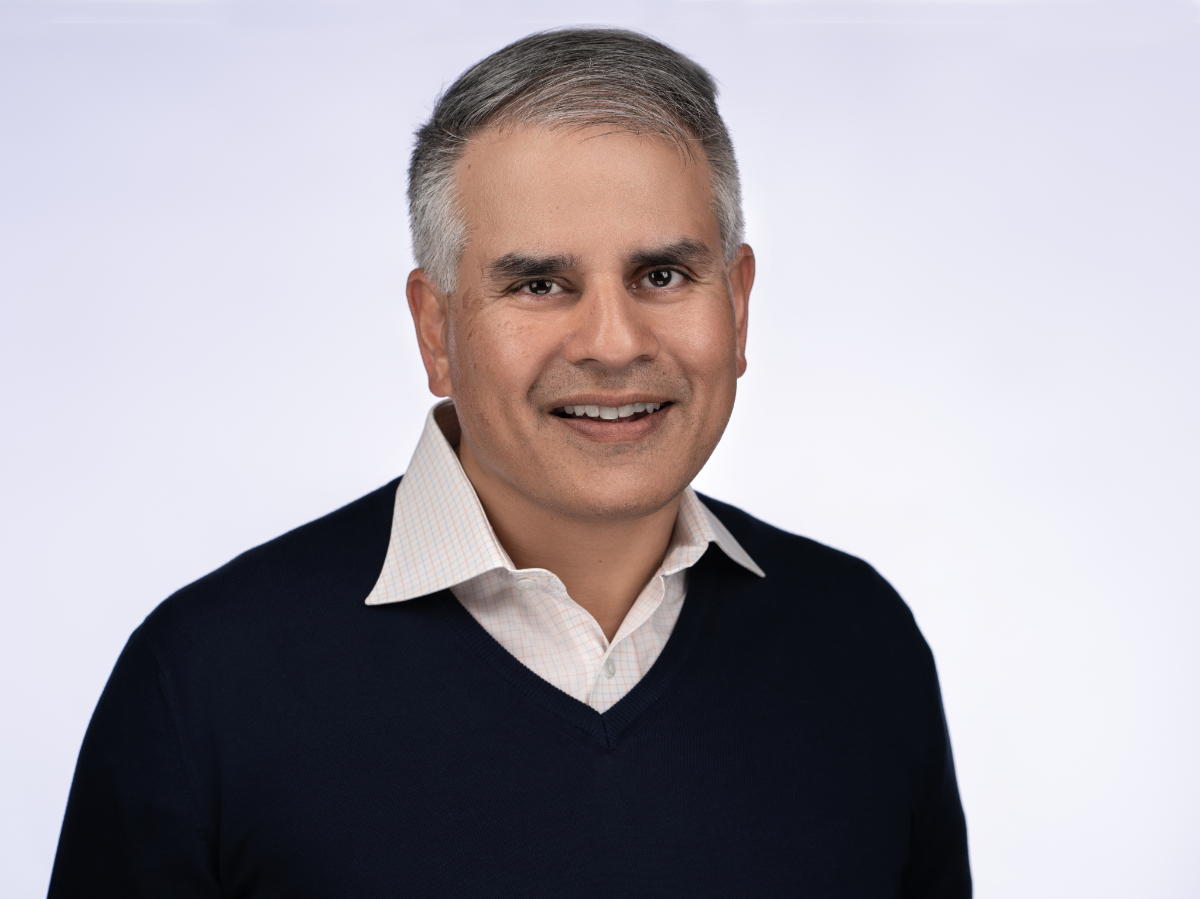
\includegraphics[width=0.3\linewidth,height=0.5\textheight]{ContributorPics/RajSahasrabuddhe} \end{center}

\begin{center}
\textbf{ Rajesh (Raj) Sahasrabuddhe }
\end{center}

\begin{itemize}
\tightlist
\item
  \textbf{Rajesh (Raj) Sahasrabuddhe} is a Partner and Philadelphia Office Leader with Oliver Wyman Actuarial Consulting. Raj is a Fellow of the Casualty Actuarial Society (CAS), an Associate of the Canadian Institute of Actuaries, and a Member of the American Academy of Actuaries. Raj has been an active volunteer with CAS Admissions committees throughout his career, including a term as Chairperson of the Syllabus Committee from 2010 to 2013. He currently serves on the MAS-II Examination Committee. He has authored or co-authored papers that have appeared on syllabi for both the CAS and Society of Actuaries.
\end{itemize}

\newpage

\begin{center}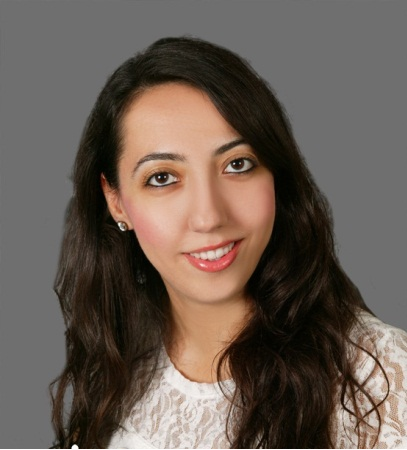
\includegraphics[width=0.2\linewidth,height=0.3\textheight]{ContributorPics/Selin_pictureA} \end{center}

\begin{center}
\textbf{ Emine Selin Sarıdaş }
\end{center}

\begin{itemize}
\tightlist
\item
  \textbf{Emine Selin Sarıdaş} is a doctoral candidate in the Statistics department of Mimar Sinan University. She holds a bachelor degree in Actuarial Science with a minor in Economics and a master degree in Actuarial Science from Hacettepe University. Her research interest includes dependence modeling, regression, loss models and life contingencies.
\end{itemize}

\begin{center}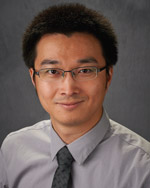
\includegraphics[width=0.2\linewidth,height=0.3\textheight]{ContributorPics/Shi_Peng_150x188} \end{center}

\begin{center}
\textbf{ Peng Shi }
\end{center}

\begin{itemize}
\tightlist
\item
  \textbf{Peng Shi} is an associate professor in the Risk and Insurance Department at the Wisconsin School of Business. He is also the Charles \& Laura Albright Professor in Business and Finance. Professor Shi is an Associate of the Casualty Actuarial Society (ACAS) and a Fellow of the Society of Actuaries (FSA). He received a Ph.D.~in actuarial science from the University of Wisconsin-Madison. His research interests are problems at the intersection of insurance and statistics. He has won several research awards, including the Charles A. Hachemeister Prize, the Ronald Bornhuetter Loss Reserve Prize, and the American Risk and Insurance Association Prize.
\end{itemize}

\newpage

\begin{center}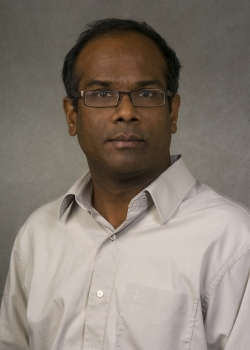
\includegraphics[width=0.2\linewidth,height=0.3\textheight]{ContributorPics/Shyamal} \end{center}

\begin{center}
\textbf{ Nariankadu D. Shyamalkumar (Shyamal) }
\end{center}

\begin{itemize}
\tightlist
\item
  \textbf{Nariankadu D. Shyamalkumar (Shyamal)} is an associate professor in the Department of Statistics and Actuarial Science at The University of Iowa. He is an Associate of the Society of Actuaries, and has volunteered in various elected and non-elected roles within the SoA. Having a broad theoretical interest as well as interest in computing, he has published in prominent actuarial, computer science, probability theory, and statistical journals. Moreover, he has worked in the financial industry, and since then served as an independent consultant to the insurance industry. He has experience educating actuaries in both Mexico and the US, serving in the roles of directing an undergraduate program, and as a graduate adviser for both masters and doctoral students.
\end{itemize}

\begin{center}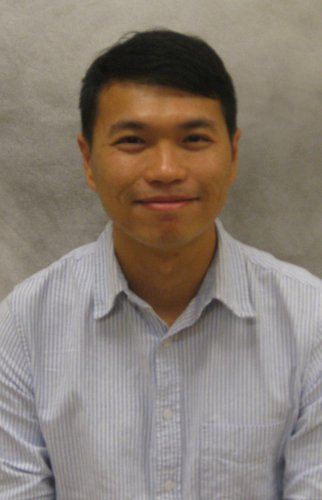
\includegraphics[width=0.2\linewidth,height=0.3\textheight]{ContributorPics/jianxi_m} \end{center}

\begin{center}
\textbf{ Jianxi Su }
\end{center}

\begin{itemize}
\tightlist
\item
  \textbf{Jianxi Su} is an Assistant Professor at the Department of Statistics at Purdue University. He is the Associate Director of Purdue's Actuarial Science. Prior to joining Purdue in 2016, he completed the PhD at York University (2012-2015). He obtained the Fellow of the Society of Actuaries (FSA) in 2017. His research expertise are in dependence modelling, risk management, and pricing. During the PhD candidature, Jianxi also worked as a research associate at the Model Validation and ORSA Implementation team of Sun Life Financial (Toronto office).
\end{itemize}

\begin{center}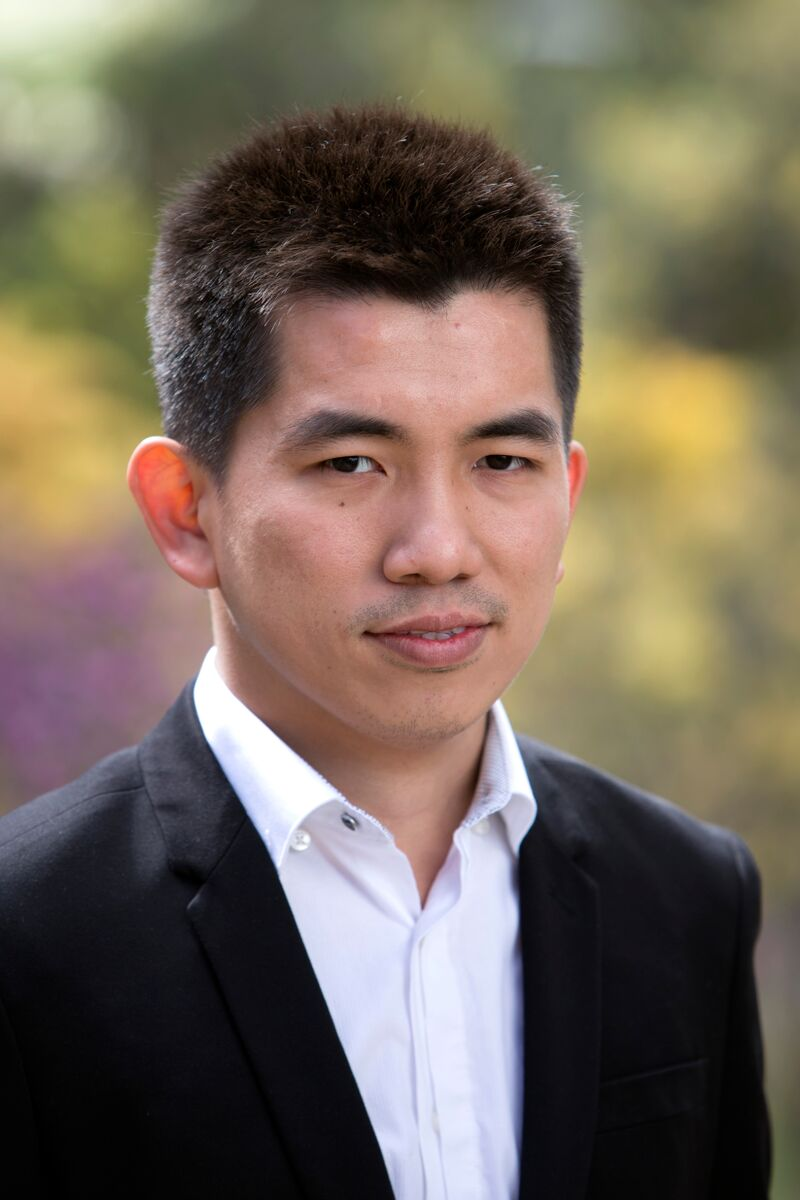
\includegraphics[width=0.2\linewidth,height=0.3\textheight]{ContributorPics/ChongItTan} \end{center}

\begin{center}
\textbf{ Chong It Tan }
\end{center}

\begin{itemize}
\tightlist
\item
  \textbf{Chong It Tan} is a senior lecturer at Macquarie University in Australia, where he has served as the undergraduate actuarial program director since 2018. He obtained his PhD in 2015 from Nanyang Technological University in Singapore. He is a fully qualified actuary, holding the credentials from both the US Society of Actuaries and Australian Actuaries Institute. His major research interests are mortality modelling, longevity risk management and bonus-malus systems.
\end{itemize}

\begin{center}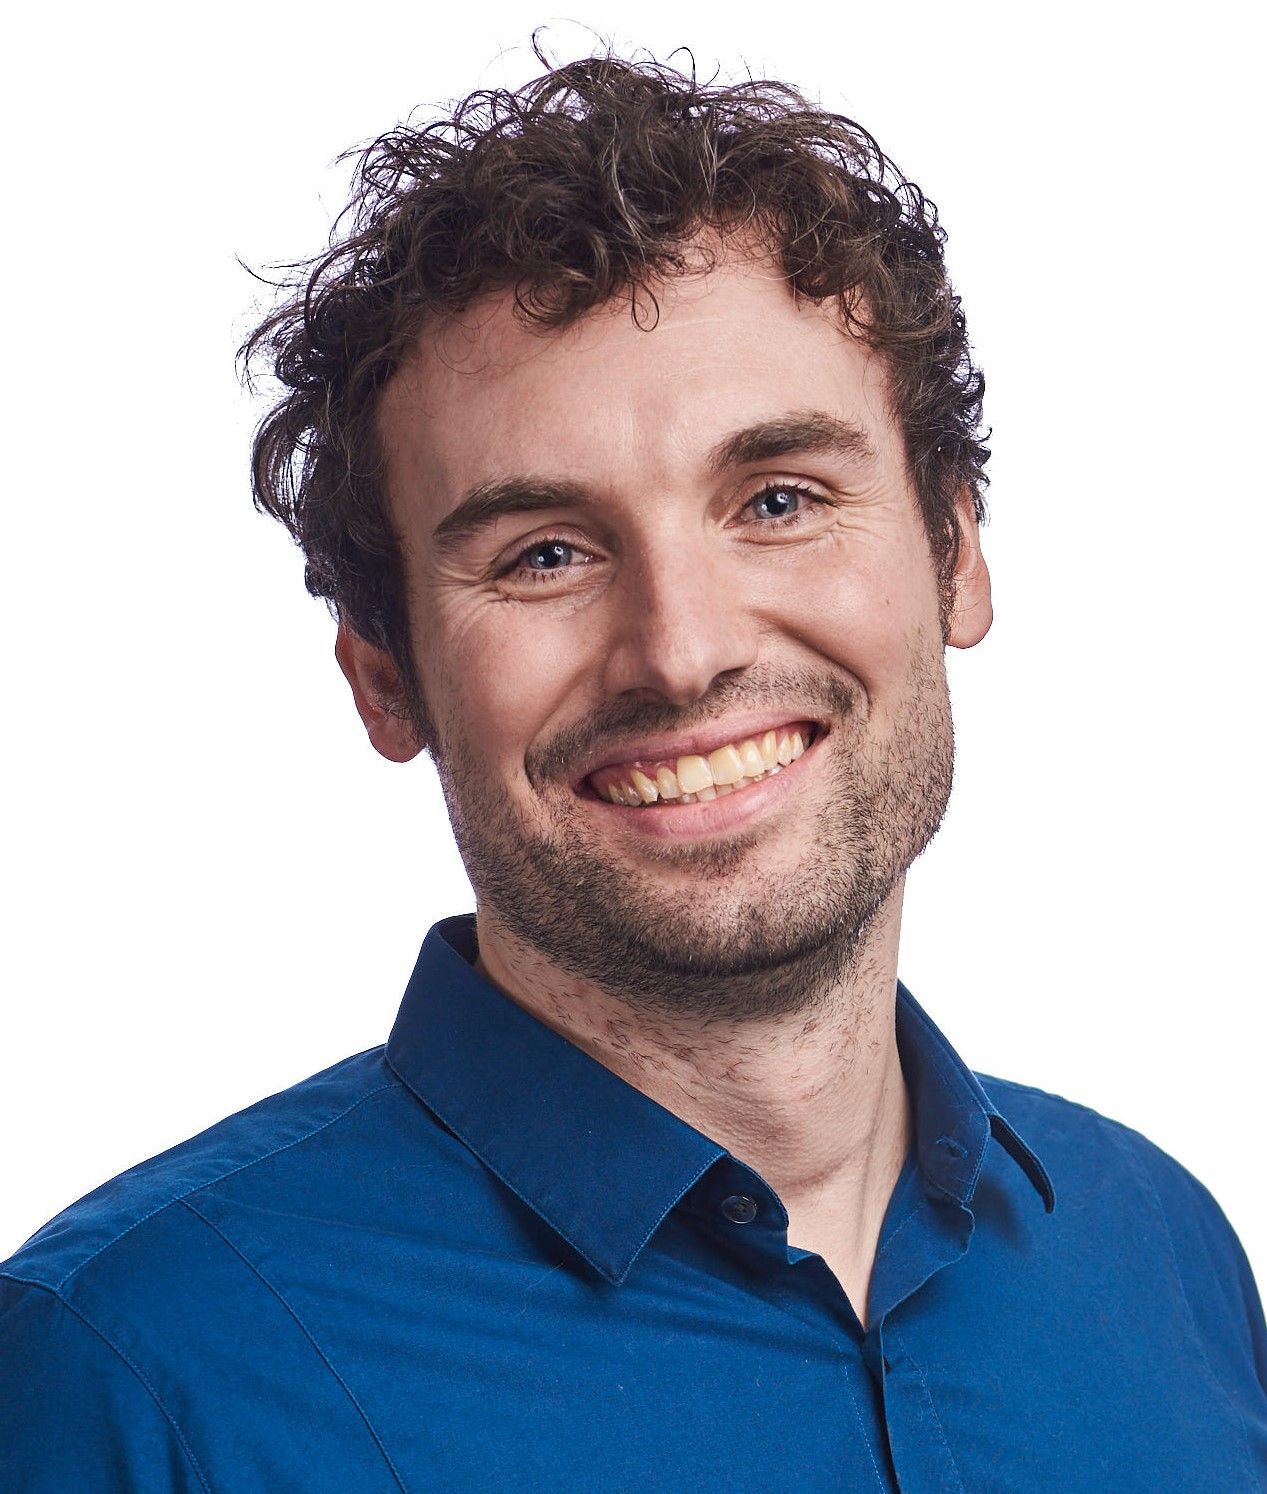
\includegraphics[width=0.2\linewidth,height=0.3\textheight]{ContributorPics/TimVerdonck} \end{center}

\begin{center}
\textbf{ Tim Verdonck }
\end{center}

\begin{itemize}
\tightlist
\item
  \textbf{Tim Verdonck} is associate professor at the University of Antwerp. He has a degree in Mathematics and a PhD in Science: Mathematics, obtained at the University of Antwerp. During his PhD he successfully took the Master in Insurance and the Master in Financial and Actuarial Engineering, both at KU Leuven. His research focuses on the adaptation and application of robust statistical methods for insurance and finance data.
\end{itemize}

\newpage

\begin{center}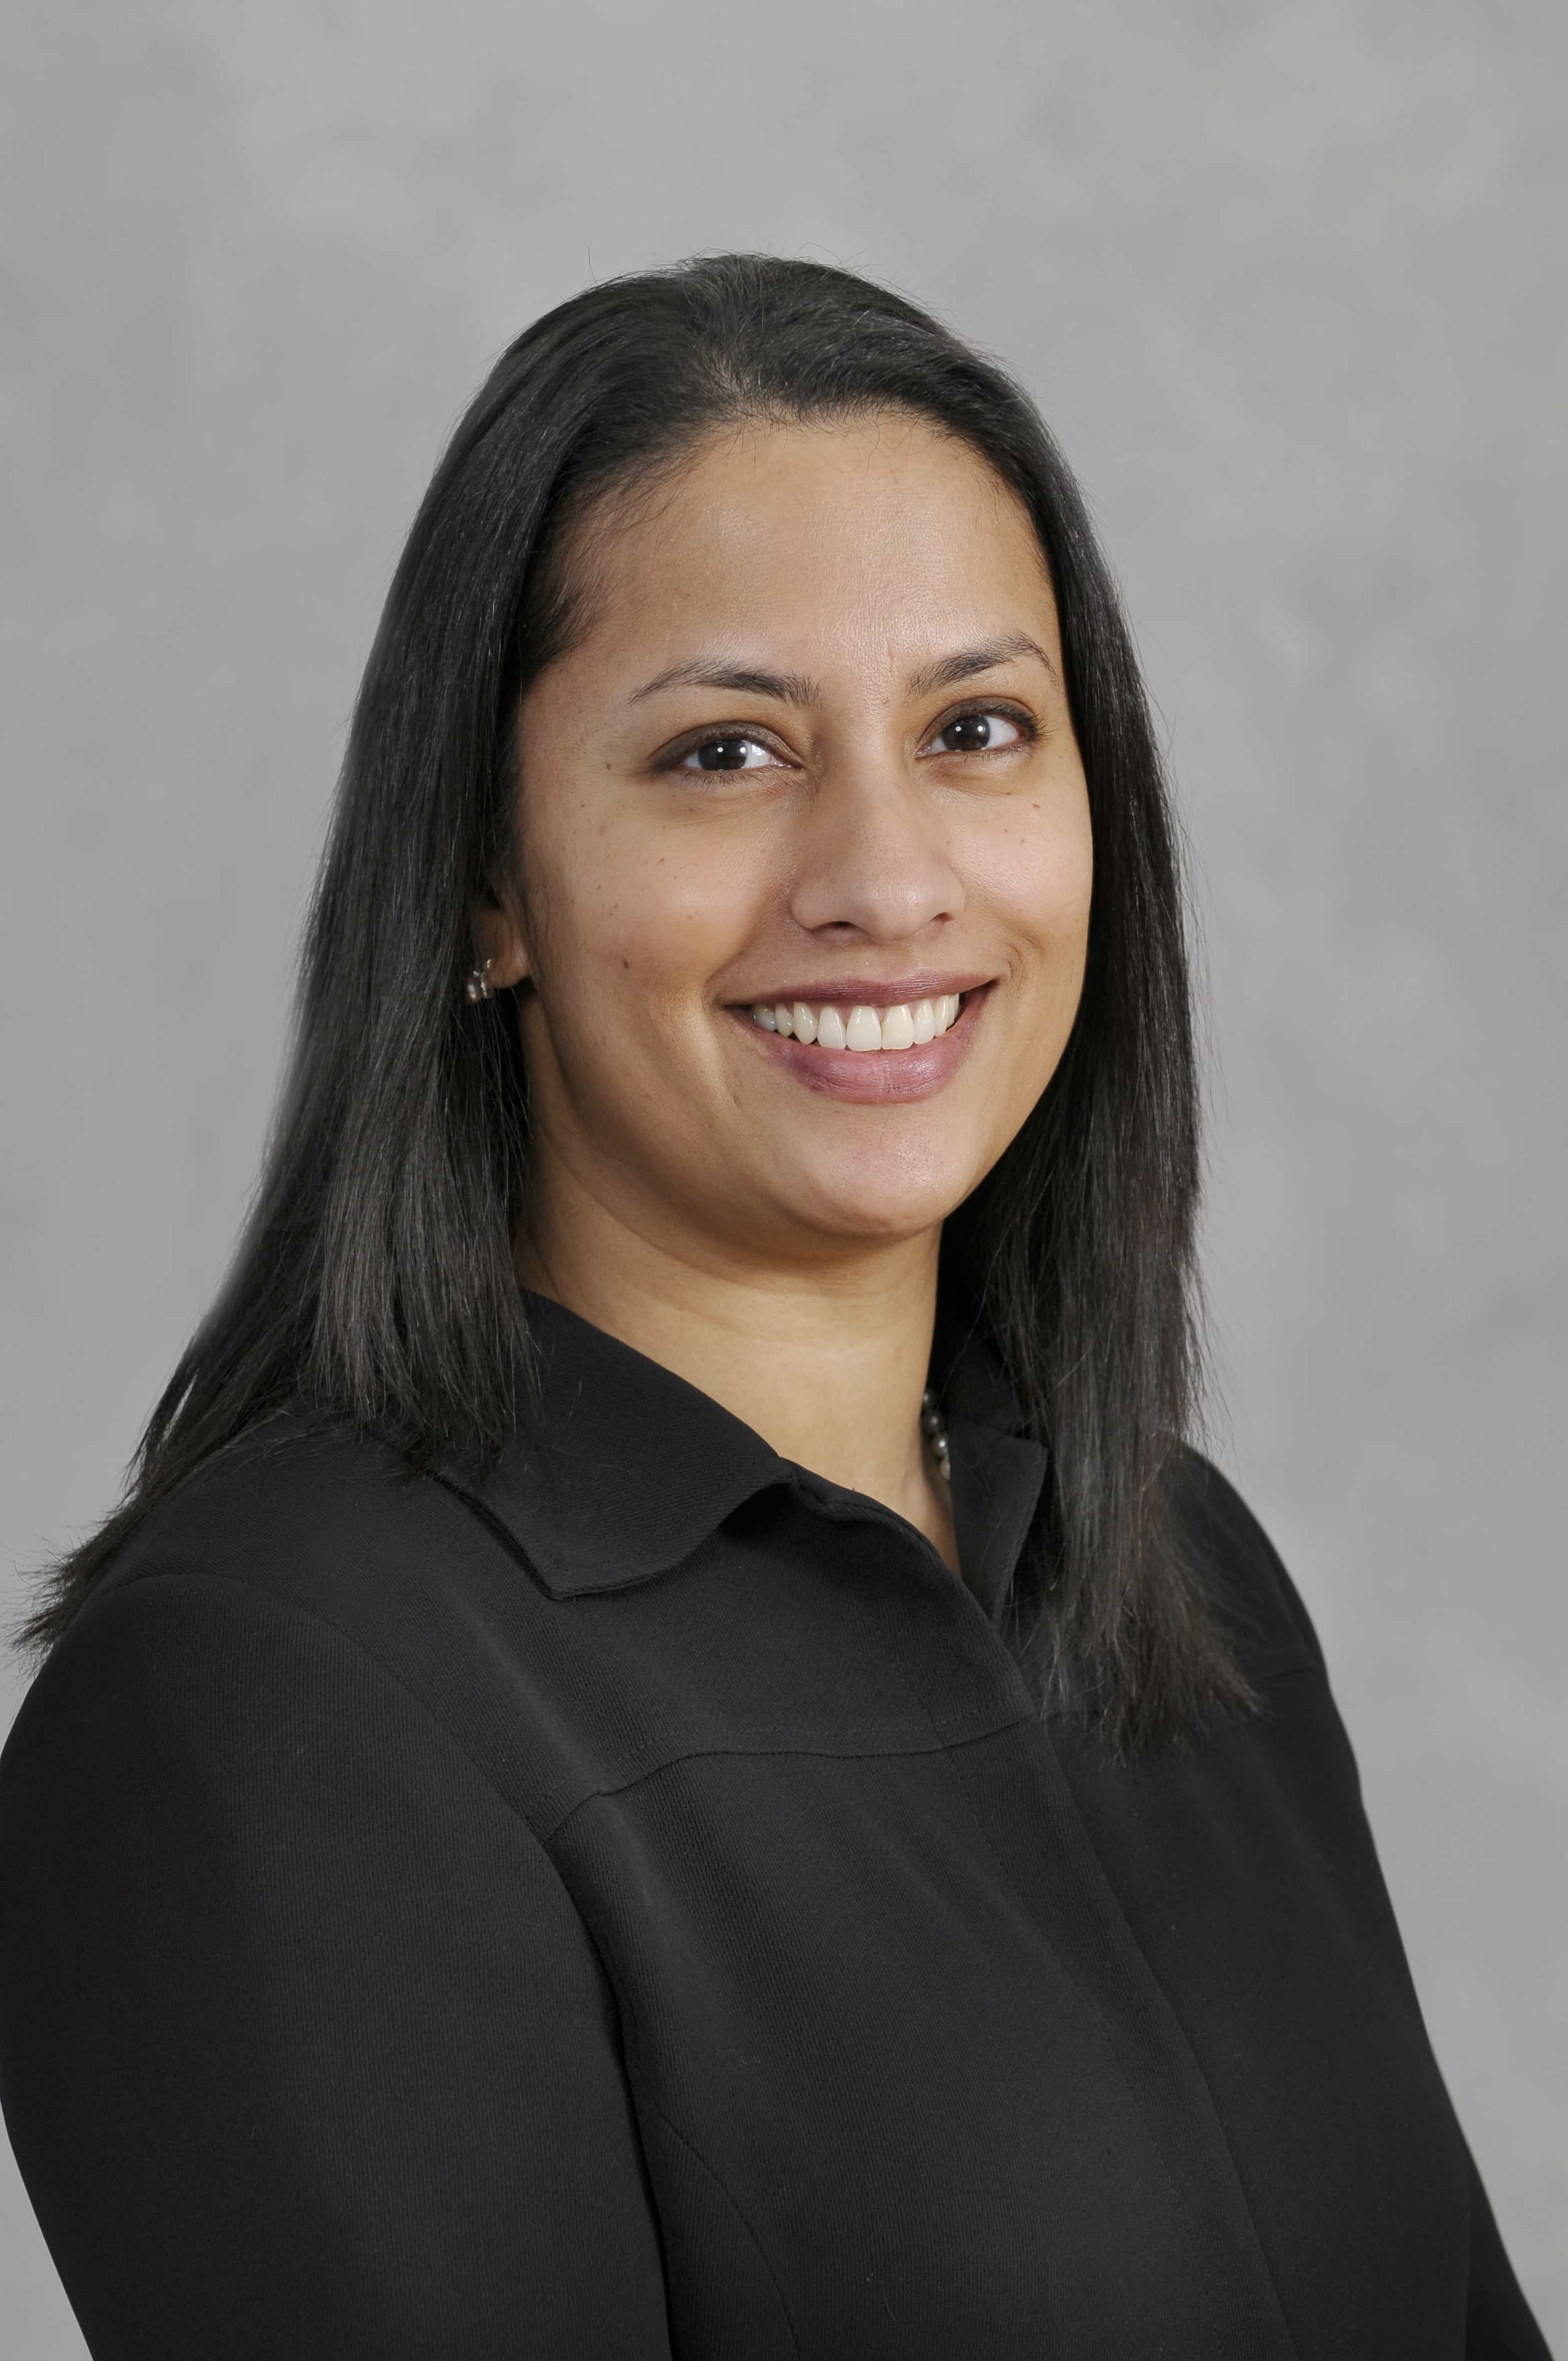
\includegraphics[width=0.2\linewidth,height=0.3\textheight]{ContributorPics/krupaviswanathan2} \end{center}

\begin{center}
\textbf{ Krupa Viswanathan }
\end{center}

\begin{itemize}
\tightlist
\item
  \textbf{Krupa Viswanathan} is an Associate Professor in the Risk, Insurance and Healthcare Management Department in the Fox School of Business, Temple University. She is an Associate of the Society of Actuaries. She teaches courses in Actuarial Science and Risk Management at the undergraduate and graduate levels. Her research interests include corporate governance of insurance companies, capital management, and sentiment analysis. She received her Ph.D.~from The Wharton School of the University of Pennsylvania.
\end{itemize}

\hypertarget{reviewers}{%
\section*{Reviewers}\label{reviewers}}


Our goal is to have the actuarial community author our textbooks in a collaborative fashion. Part of the writing process involves many reviewers who generously donated their time to help make this book better. They are:

\begin{itemize}
\tightlist
\item
  Yair Babab
\item
  David Back, Liberty Mutual
\item
  Chunsheng Ban, Ohio State University
\item
  Vytaras Brazauskas, University of Wisconsin - Milwaukee
\item
  Yvonne Chueh, Central Washington University
\item
  Chun Yong Chew, Universiti Tunku Abdul Rahman (UTAR)
\item
  Benjamin Côté, Université Laval
\item
  Eren Dodd, University of Southampton
\item
  Gordon Enderle, University of Wisconsin - Madison
\item
  Rob Erhardt, Wake Forest University
\item
  Runhun Feng, University of Illinois
\item
  Brian Hartman, Brigham Young University
\item
  Liang (Jason) Hong, University of Texas at Dallas
\item
  Fei Huang, Australian National University
\item
  Hirokazu (Iwahiro) Iwasawa
\item
  Himchan Jeong, University of Connecticut
\item
  Min Ji, Towson University
\item
  Paul Herbert Johnson, University of Wisconsin - Madison
\item
  Dalia Khalil, Cairo University
\item
  Samuel Kolins, Lebonan Valley College
\item
  Andrew Kwon-Nakamura, Zurich North America
\item
  Ambrose Lo, University of Iowa
\item
  Mélina Mailhot, Concordia University
\item
  Mark Maxwell, University of Texas at Austin
\item
  Tatjana Miljkovic, Miami University
\item
  Bell Ouelega, American University in Cairo
\item
  Zhiyu (Frank) Quan, University of Connecticut
\item
  Jiandong Ren, Western University
\item
  Margie Rosenberg, University of Wisconsin - Madison
\item
  Rajesh V. Sahasrabuddhe, Oliver Wyman
\item
  Sherly Paola Alfonso Sanchez, Universidad Nacional de Colombia
\item
  Ranee Thiagarajah, Illinois State University
\item
  Ping Wang, Saint Johns University
\item
  Chengguo Weng, University of Waterloo
\item
  Toby White, Drake University
\item
  Michelle Xia, Northern Illinois University
\item
  Di (Cindy) Xu, University of Nebraska - Lincoln
\item
  Lina Xu, Columbia University
\item
  Lu Yang, University of Amsterdam
\item
  Chun Yong
\item
  Jorge Yslas, University of Copenhagen
\item
  Jeffrey Zheng, Temple University
\item
  Hongjuan Zhou, Arizona State University
\end{itemize}

\hypertarget{other-collaborators}{%
\subsection*{Other Collaborators}\label{other-collaborators}}


\begin{itemize}
\tightlist
\item
  Alyaa Nuval Binti Othman, Aisha Nuval Binti Othman, and Khairina (Rina) Binti Ibraham were three of many students at the Univeristy of Wiscinson-Madison that helped with the text over the years.
\item
  Maggie Lee, Macquarie University, and Anh Vu (then at University of New South Wales) contributed the end of the section quizzes.
\item
  Jeffrey Zheng, Temple University, Lu Yang (University of Amsterdam), and Paul Johnson, University of Wisconsin-Madison, led the work on the glossary.
\end{itemize}

\hypertarget{version-number}{%
\section*{Version Number}\label{version-number}}


\begin{itemize}
\tightlist
\item
  This is \textbf{Version 2.0}, October 2024. Edited by Hélène Cossette, Edward (Jed) Frees, Brian Hartman, and Tim Higgins.
\item
  Version 1.1, August 2020. Edited by Edward (Jed) Frees and Paul Johnson.
\item
  Version 1.0, January 2020, was edited by Edward (Jed) Frees.
\end{itemize}

You can also access pdf and epub (current and older) versions of the text in our \href{https://ewfrees.github.io/Loss-Data-Analytics/DownloadOffline.html}{Offline versions of the text}.

\hypertarget{for-our-readers}{%
\section*{For our Readers}\label{for-our-readers}}


We hope that you find this book worthwhile and even enjoyable. For your convenience, at our \href{https://openacttexts.github.io/}{Github Landing site} (\url{https://openacttexts.github.io/}), you will find links to the book that you can (freely) download for offline reading, including a pdf version (for Adobe Acrobat) and an EPUB version suitable for mobile devices. \href{https://github.com/OpenActTexts/Loss-Data-Analytics/tree/master/Data}{Data} for running our examples are available at the same site.

In developing this book, we are emphasizing the \href{https://openacttexts.github.io/Loss-Data-Analytics/index.html}{online version} that has lots of great features such as a glossary, code and solutions to examples that you can be revealed interactively. For example, you will find that the statistical code is hidden and can only be seen by clicking on terms such as

We hide the code because we don't want to insist that you use the \texttt{R} statistical software (although we like it). Still, we encourage you to try some statistical code as you read the book -- we have opted to make it easy to learn \texttt{R} as you go. We have set up a separate \href{https://openacttexts.github.io/LDARcode}{R Code for Loss Data Analytics} site to explain more of the details of the code.

Like any book, we have a set of notations and conventions. It will probably save you time if you regularly visit our Appendix Chapter \ref{ChapNotationConvention} to get used to ours.

Freely available, interactive textbooks represent a new venture in actuarial education and we need your input. Although a lot of effort has gone into the development, we expect hiccoughs. Please let your instructor know about opportunities for improvement, write us through our project site, or contact chapter contributors directly with suggested improvements.

\begin{center}\rule{0.5\linewidth}{0.5pt}\end{center}

This work is licensed under a Creative Commons Attribution 4.0 International License.

\mainmatter

\hypertarget{DataResources}{%
\chapter{Appendix. Data Resources}\label{DataResources}}

This appendix section describes the datasets used in this book and others that you may wish to explore.

For each set of data, we provide download buttons so that you can easily access the data in standard .csv (comma separated value) format. This allows you replicate and experiment with the methods developed in the book as well as sharpen your understanding through exercises.

We provide the source of each dataset. We also recommend, for deeper understanding, that you occasionally refer to these original sources to further develop your appreciation of the data underpinning the analytics developed in this book.

\hypertarget{S:WiscPropFundA}{%
\section{Wisconsin Property Fund}\label{S:WiscPropFundA}}

\textbf{Description}: The Wisconsin Local Government Property Insurance Fund (LGPIF) is an insurance pool administered by the Wisconsin Office of the Insurance Commissioner. The LGPIF was established to provide property insurance for local government entities that include counties, cities, towns, villages, school districts, and library boards. The fund insures local government property such as government buildings, schools, libraries, and motor vehicles. It covers all property losses except those resulting from flood, earthquake, wear and tear, extremes in temperature, mold, war, nuclear reactions, and embezzlement or theft by an employee.

The data are available using this download button:
Download the Wisconsin Property Fund Data

\begin{table}[!h]
\centering\centering
\caption{\label{tab:unnamed-chunk-30}\textbf{Variables in the Wisconsin Property Fund Dataset}}
\centering
\fontsize{10}{12}\selectfont
\begin{tabular}[t]{>{}l>{\raggedright\arraybackslash}p{12cm}}
\toprule
Variable & Description\\
\midrule
\cellcolor{gray!10}{PolicyNum} & \cellcolor{gray!10}{Policy number}\\
Year & Contract year\\
\cellcolor{gray!10}{Premium} & \cellcolor{gray!10}{Premium}\\
Deduct & Deductible\\
\cellcolor{gray!10}{BCcov} & \cellcolor{gray!10}{Coverage for building and contents}\\
\addlinespace
Freq & Number of claims during the year (frequency)\\
\cellcolor{gray!10}{Fire5} & \cellcolor{gray!10}{Binary variable to indicate the fire class is below 5}\\
NoClaimCredit & Binary variable to indicate no claims in the past two years\\
\cellcolor{gray!10}{EntityType} & \cellcolor{gray!10}{Categorical variable that is one of six types:  1=Village, 2=City,3=County, 4=Misc, 5=School, or Town)}\\
AlarmCredit & Categorical variable that is one of four types:  (0, 5, 10, or 15) for automatic smoke alarms in main rooms\\
\addlinespace
\cellcolor{gray!10}{BCClaim} & \cellcolor{gray!10}{Builing and contents claims}\\
\bottomrule
\end{tabular}
\end{table}

\begin{table}[!h]
\centering\centering
\caption{\label{tab:unnamed-chunk-31}\textbf{Wisconsin Property Fund First Five Rows}}
\centering
\fontsize{6}{8}\selectfont
\begin{tabular}[t]{>{}c>{\centering\arraybackslash}p{0.7cm}>{\centering\arraybackslash}p{0.7cm}>{\centering\arraybackslash}p{0.7cm}>{\centering\arraybackslash}p{1.0cm}>{\centering\arraybackslash}p{0.7cm}>{\centering\arraybackslash}p{0.7cm}>{\centering\arraybackslash}p{1.4cm}>{\centering\arraybackslash}p{1.0cm}>{\centering\arraybackslash}p{1.0cm}>{\centering\arraybackslash}p{1.0cm}>{}p{0.7cm}}
\toprule
PolicyNum & Year & Premium & Deduct & BCcov & Freq & Fire5 & NoClaimCredit & EntityType & AlarmCredit & BCClaim\\
\midrule
\cellcolor{gray!10}{120002} & \cellcolor{gray!10}{2006} & \cellcolor{gray!10}{9313} & \cellcolor{gray!10}{1000} & \cellcolor{gray!10}{22714456} & \cellcolor{gray!10}{0} & \cellcolor{gray!10}{1} & \cellcolor{gray!10}{0} & \cellcolor{gray!10}{3} & \cellcolor{gray!10}{1} & \cellcolor{gray!10}{0}\\
120002 & 2007 & 8767 & 1000 & 25046646 & 0 & 1 & 0 & 3 & 1 & 0\\
\cellcolor{gray!10}{120002} & \cellcolor{gray!10}{2008} & \cellcolor{gray!10}{7090} & \cellcolor{gray!10}{1000} & \cellcolor{gray!10}{20851525} & \cellcolor{gray!10}{0} & \cellcolor{gray!10}{1} & \cellcolor{gray!10}{1} & \cellcolor{gray!10}{3} & \cellcolor{gray!10}{1} & \cellcolor{gray!10}{0}\\
120002 & 2009 & 8522 & 1000 & 21852696 & 0 & 1 & 1 & 3 & 1 & 0\\
\cellcolor{gray!10}{120002} & \cellcolor{gray!10}{2010} & \cellcolor{gray!10}{7994} & \cellcolor{gray!10}{1000} & \cellcolor{gray!10}{23511493} & \cellcolor{gray!10}{1} & \cellcolor{gray!10}{1} & \cellcolor{gray!10}{1} & \cellcolor{gray!10}{3} & \cellcolor{gray!10}{1} & \cellcolor{gray!10}{6839}\\
\bottomrule
\end{tabular}
\end{table}

\begin{table}[!h]
\centering\centering
\caption{\label{tab:unnamed-chunk-31}\textbf{Wisconsin Property Fund Last Five Rows}}
\centering
\fontsize{6}{8}\selectfont
\begin{tabular}[t]{>{}c>{\centering\arraybackslash}p{0.7cm}>{\centering\arraybackslash}p{0.7cm}>{\centering\arraybackslash}p{0.7cm}>{\centering\arraybackslash}p{1.0cm}>{\centering\arraybackslash}p{0.7cm}>{\centering\arraybackslash}p{0.7cm}>{\centering\arraybackslash}p{1.4cm}>{\centering\arraybackslash}p{1.0cm}>{\centering\arraybackslash}p{1.0cm}>{\centering\arraybackslash}p{1.0cm}>{}p{0.7cm}}
\toprule
PolicyNum & Year & Premium & Deduct & BCcov & Freq & Fire5 & NoClaimCredit & EntityType & AlarmCredit & BCClaim\\
\midrule
\cellcolor{gray!10}{180787} & \cellcolor{gray!10}{2010} & \cellcolor{gray!10}{199} & \cellcolor{gray!10}{500} & \cellcolor{gray!10}{285000} & \cellcolor{gray!10}{0} & \cellcolor{gray!10}{1} & \cellcolor{gray!10}{1} & \cellcolor{gray!10}{4} & \cellcolor{gray!10}{1} & \cellcolor{gray!10}{0}\\
180788 & 2010 & 58344 & 100000 & 416739800 & 1 & 1 & 0 & 4 & 1 & 168304\\
\cellcolor{gray!10}{180789} & \cellcolor{gray!10}{2010} & \cellcolor{gray!10}{295} & \cellcolor{gray!10}{500} & \cellcolor{gray!10}{500988} & \cellcolor{gray!10}{1} & \cellcolor{gray!10}{1} & \cellcolor{gray!10}{0} & \cellcolor{gray!10}{4} & \cellcolor{gray!10}{1} & \cellcolor{gray!10}{1034}\\
180790 & 2010 & 2077 & 1000 & 3580665 & 0 & 1 & 0 & 4 & 4 & 0\\
\cellcolor{gray!10}{180791} & \cellcolor{gray!10}{2010} & \cellcolor{gray!10}{81} & \cellcolor{gray!10}{500} & \cellcolor{gray!10}{118800} & \cellcolor{gray!10}{0} & \cellcolor{gray!10}{1} & \cellcolor{gray!10}{0} & \cellcolor{gray!10}{4} & \cellcolor{gray!10}{1} & \cellcolor{gray!10}{0}\\
\bottomrule
\end{tabular}
\end{table}

\hypertarget{Sec:DataTravel}{%
\section{ANU Corporate Travel Data}\label{Sec:DataTravel}}

Universities purchase corporate travel policies to cover employees and students traveling on official university business for a wide variety of accidents and incidents while away from the campus or primary workplace. This broad coverage includes medical care and evacuation, loss of personal property, extraction for political and weather related reasons, and more. See \citet{frees2022ANURisks} for more information about this coverage.

There are 2107 observations in this dataset. The variable names are described in Table \ref{tab:DescribeTravel} and the first and last five observations are in Table \ref{tab:PrintNumTravel}.

Data are available using this button:
Download Corporate Travel Claims Data.

\begin{table}[!h]
\centering\centering
\caption{\label{tab:DescribeTravel}\textbf{Variables in the Corporate Travel Dataset}}
\centering
\fontsize{10}{12}\selectfont
\begin{tabular}[t]{>{}l>{\raggedright\arraybackslash}p{12cm}}
\toprule
Variable & Description\\
\midrule
\cellcolor{gray!10}{UW Year} & \cellcolor{gray!10}{Underwriting Year}\\
Loss Date & Date that the loss occurred\\
\cellcolor{gray!10}{Reported Date} & \cellcolor{gray!10}{Date that the loss was reported}\\
Last Trans Date & Last date in which there was a transaction regarding the loss\\
\cellcolor{gray!10}{Paid Loss} & \cellcolor{gray!10}{Cumulative amount paid on the loss}\\
\addlinespace
Outstanding Reserve & Estimate of the loss amount yet to be paid\\
\cellcolor{gray!10}{Incurred Loss} & \cellcolor{gray!10}{Sum of the amount paid and the estimate of future payments}\\
Status & An indicator as to whether the claim has been deemed settled (closed) or not settled (open)\\
\bottomrule
\end{tabular}
\end{table}

\begin{table}[!h]
\centering\centering
\caption{\label{tab:PrintNumTravel}\textbf{Corporate Travel Data First Five Rows}}
\centering
\fontsize{6}{8}\selectfont
\begin{tabular}[t]{>{}c>{\centering\arraybackslash}p{1.4cm}>{\centering\arraybackslash}p{1.4cm}>{\centering\arraybackslash}p{1.4cm}>{\centering\arraybackslash}p{1.4cm}>{\centering\arraybackslash}p{2.4cm}>{\centering\arraybackslash}p{1.4cm}>{\centering\arraybackslash}p{1.4cm}>{}p{1.4cm}}
\toprule
UW.Year & Loss.Date & Reported.Date & Last.Trans.Date & Paid.Loss & Outstanding.Reserve & Incurred.Loss & Status\\
\midrule
\cellcolor{gray!10}{2021} & \cellcolor{gray!10}{19/12/2021} & \cellcolor{gray!10}{20/12/2021} & \cellcolor{gray!10}{24/12/2021} & \cellcolor{gray!10}{10000} & \cellcolor{gray!10}{0} & \cellcolor{gray!10}{10000} & \cellcolor{gray!10}{Closed}\\
2021 & 9/4/2022 & 29/04/2022 & 30/05/2022 & 423 & 0 & 423 & Closed\\
\cellcolor{gray!10}{2021} & \cellcolor{gray!10}{2/5/2022} & \cellcolor{gray!10}{4/5/2022} & \cellcolor{gray!10}{} & \cellcolor{gray!10}{0} & \cellcolor{gray!10}{500} & \cellcolor{gray!10}{500} & \cellcolor{gray!10}{Open}\\
2021 & 5/5/2022 & 17/05/2022 &  & 0 & 562 & 562 & Open\\
\cellcolor{gray!10}{2021} & \cellcolor{gray!10}{30/04/2022} & \cellcolor{gray!10}{27/05/2022} & \cellcolor{gray!10}{10/6/2022} & \cellcolor{gray!10}{1500} & \cellcolor{gray!10}{0} & \cellcolor{gray!10}{1500} & \cellcolor{gray!10}{Closed}\\
\bottomrule
\end{tabular}
\end{table}

\begin{table}[!h]
\centering\centering
\caption{\label{tab:PrintNumTravel}\textbf{Corporate Travel Data Last Five Rows}}
\centering
\fontsize{6}{8}\selectfont
\begin{tabular}[t]{>{}c>{\centering\arraybackslash}p{1.4cm}>{\centering\arraybackslash}p{1.4cm}>{\centering\arraybackslash}p{1.4cm}>{\centering\arraybackslash}p{1.4cm}>{\centering\arraybackslash}p{2.4cm}>{\centering\arraybackslash}p{1.4cm}>{\centering\arraybackslash}p{1.4cm}>{}p{1.4cm}}
\toprule
UW.Year & Loss.Date & Reported.Date & Last.Trans.Date & Paid.Loss & Outstanding.Reserve & Incurred.Loss & Status\\
\midrule
\cellcolor{gray!10}{2006} & \cellcolor{gray!10}{1/11/2006} & \cellcolor{gray!10}{19/06/2007} & \cellcolor{gray!10}{} & \cellcolor{gray!10}{0} & \cellcolor{gray!10}{0} & \cellcolor{gray!10}{0} & \cellcolor{gray!10}{Closed}\\
2006 & 24/06/2007 & 26/06/2007 & 8/1/2008 & 6278 & 0 & 6278 & Closed\\
\cellcolor{gray!10}{2006} & \cellcolor{gray!10}{4/7/2007} & \cellcolor{gray!10}{6/7/2007} & \cellcolor{gray!10}{11/9/2007} & \cellcolor{gray!10}{114} & \cellcolor{gray!10}{0} & \cellcolor{gray!10}{114} & \cellcolor{gray!10}{Closed}\\
2006 & 20/05/2007 & 26/06/2007 & 14/07/2007 & 136 & 0 & 136 & Closed\\
\cellcolor{gray!10}{2006} & \cellcolor{gray!10}{15/02/2007} & \cellcolor{gray!10}{27/06/2007} & \cellcolor{gray!10}{14/07/2007} & \cellcolor{gray!10}{1208} & \cellcolor{gray!10}{0} & \cellcolor{gray!10}{1208} & \cellcolor{gray!10}{Closed}\\
\bottomrule
\end{tabular}
\end{table}

\emph{Source}: Frees, Edward and Butt, Adam (2022). ``ANU Corporate Travel Insurance Claims 2022''. Australian National University Data Commons. DOI \url{https://doi.org/10.25911/vrdw-9f32}.

\hypertarget{Sec:DataGPA}{%
\section{ANU Group Personal Accident Data}\label{Sec:DataGPA}}

Group personal accident insurance offers financial protection in case of injury or death resulting from an incident that occurs on the job. Like workers' compensation, group personal accident offers insurance coverage and liability insurance protection against accidental death or injury. Unlike workers' compensation, group personal accident covers students and ANU's voluntary workers. See \citet{frees2022ANURisks} for more information about this coverage.

There are 148 observations in this dataset. The variable names are described in Table \ref{tab:DescribeGPA} and the first and last five observations are in Table \ref{tab:PrintNumGPA}.

Data are available using this button: Download Group Personal Accident Claims Data.

\begin{table}[!h]
\centering\centering
\caption{\label{tab:DescribeGPA}\textbf{Variables in the Group Personal Accident Dataset}}
\centering
\fontsize{10}{12}\selectfont
\begin{tabular}[t]{>{}l>{\raggedright\arraybackslash}p{12cm}}
\toprule
Variable & Description\\
\midrule
\cellcolor{gray!10}{UW Year} & \cellcolor{gray!10}{Underwriting Year}\\
Loss Date & Date that the loss occurred\\
\cellcolor{gray!10}{Last Trans Date} & \cellcolor{gray!10}{Last date in which there was a transaction regarding the loss.}\\
Paid Loss & Cumulative amount paid on the loss\\
\cellcolor{gray!10}{Outstanding Reserve} & \cellcolor{gray!10}{Estimate of the loss amount yet to be paid}\\
\addlinespace
Incurred Loss & Sum of the amount paid and the estimate of future payments\\
\cellcolor{gray!10}{Status} & \cellcolor{gray!10}{An indicator as to whether the claim has been deemed settled (closed) or not settled (open)}\\
\bottomrule
\end{tabular}
\end{table}

\begin{table}[!h]
\centering\centering
\caption{\label{tab:PrintNumGPA}\textbf{Group Personal Accident  Data First Five Rows}}
\centering
\fontsize{6}{8}\selectfont
\begin{tabular}[t]{>{}c>{\centering\arraybackslash}p{1.3cm}>{\centering\arraybackslash}p{1.3cm}>{\centering\arraybackslash}p{1.3cm}>{\centering\arraybackslash}p{1.6cm}>{\centering\arraybackslash}p{1.3cm}>{\centering\arraybackslash}p{1.3cm}>{}p{1.3cm}}
\toprule
UW.Year & Loss.Date & Last.Trans.Date & Paid.Loss & Outstanding.Reserve & Incurred.Loss & Status\\
\midrule
\cellcolor{gray!10}{2021} & \cellcolor{gray!10}{6/12/2021} & \cellcolor{gray!10}{3/6/2022} & \cellcolor{gray!10}{805} & \cellcolor{gray!10}{0} & \cellcolor{gray!10}{805} & \cellcolor{gray!10}{Closed}\\
2021 & 15/11/2021 &  & 0 & 0 & 0 & \vphantom{1} Closed\\
\cellcolor{gray!10}{2021} & \cellcolor{gray!10}{15/11/2021} & \cellcolor{gray!10}{} & \cellcolor{gray!10}{0} & \cellcolor{gray!10}{0} & \cellcolor{gray!10}{0} & \cellcolor{gray!10}{Closed}\\
2021 & 22/03/2022 & 4/5/2022 & 396 & 0 & 396 & Closed\\
\cellcolor{gray!10}{2021} & \cellcolor{gray!10}{11/4/2022} & \cellcolor{gray!10}{2/8/2022} & \cellcolor{gray!10}{740} & \cellcolor{gray!10}{360} & \cellcolor{gray!10}{1100} & \cellcolor{gray!10}{Open}\\
\bottomrule
\end{tabular}
\end{table}

\begin{table}[!h]
\centering\centering
\caption{\label{tab:PrintNumGPA}\textbf{Group Personal Accident  Data Last Five Rows}}
\centering
\fontsize{6}{8}\selectfont
\begin{tabular}[t]{>{}c>{\centering\arraybackslash}p{1.3cm}>{\centering\arraybackslash}p{1.3cm}>{\centering\arraybackslash}p{1.3cm}>{\centering\arraybackslash}p{1.6cm}>{\centering\arraybackslash}p{1.3cm}>{\centering\arraybackslash}p{1.3cm}>{}p{1.3cm}}
\toprule
UW.Year & Loss.Date & Last.Trans.Date & Paid.Loss & Outstanding.Reserve & Incurred.Loss & Status\\
\midrule
\cellcolor{gray!10}{2010} & \cellcolor{gray!10}{6/3/2011} & \cellcolor{gray!10}{26/07/2011} & \cellcolor{gray!10}{776} & \cellcolor{gray!10}{0} & \cellcolor{gray!10}{776} & \cellcolor{gray!10}{Closed}\\
2010 & 22/07/2011 & 23/01/2012 & 4625 & 0 & 4625 & Closed\\
\cellcolor{gray!10}{2010} & \cellcolor{gray!10}{5/6/2011} & \cellcolor{gray!10}{30/01/2012} & \cellcolor{gray!10}{1504} & \cellcolor{gray!10}{0} & \cellcolor{gray!10}{1504} & \cellcolor{gray!10}{Closed}\\
2007 & 11/1/2008 & 23/02/2008 & 0 & 0 & 0 & Closed\\
\cellcolor{gray!10}{2007} & \cellcolor{gray!10}{29/08/2008} & \cellcolor{gray!10}{} & \cellcolor{gray!10}{0} & \cellcolor{gray!10}{0} & \cellcolor{gray!10}{0} & \cellcolor{gray!10}{Closed}\\
\bottomrule
\end{tabular}
\end{table}

\emph{Source}: Frees, Edward and Butt, Adam (2022). ``ANU Group Personal Accident Claims 2022''. Australian National University Data Commons. \url{https://doi.org/10.25911/jcfx-zj56}.

\hypertarget{Sec:DataAuto}{%
\section{ANU Motor Vehicle Data}\label{Sec:DataAuto}}

This policy covers ANU's vehicles including cars, vans, utilities, and motorcycles. See \citet{frees2022ANURisks} for more information about this coverage.

There are 318 observations in this dataset. The variable names are described in Table \ref{tab:DescribeAuto} and the first and last five observations are in Table \ref{tab:PrintNumAuto}.

Data are available using this button:
Download Motor Vehicle Claims Data.

\begin{table}[!h]
\centering\centering
\caption{\label{tab:DescribeAuto}\textbf{Variables in the Motor Vehicle Dataset}}
\centering
\fontsize{10}{12}\selectfont
\begin{tabular}[t]{>{}l>{\raggedright\arraybackslash}p{12cm}}
\toprule
Variable & Description\\
\midrule
\cellcolor{gray!10}{Policy Term Start Date} & \cellcolor{gray!10}{Start date of the contract year in which the loss occurred}\\
Loss Date & Date that the loss occurred\\
\cellcolor{gray!10}{Reported Date} & \cellcolor{gray!10}{Date that the loss was reported}\\
Motor Fault & Party responsible for the loss\\
\cellcolor{gray!10}{Driver Age} & \cellcolor{gray!10}{Age of the driver}\\
\addlinespace
Vehicle Description & Type of vehicle\\
\cellcolor{gray!10}{Loss Postcode} & \cellcolor{gray!10}{Postal code where the loss occurred}\\
Excess & The deductible applied to the loss\\
\cellcolor{gray!10}{Motor Net Paid} & \cellcolor{gray!10}{Amount paid to the insured (ANU)}\\
Outstanding Estimate & Estimate of the loss amount yet to be paid\\
\addlinespace
\cellcolor{gray!10}{Motor Net Incurred} & \cellcolor{gray!10}{Sum of the amount paid and the estimate of future payments}\\
Third Party Identified & Indicates whether a responsible third party could be identified\\
\cellcolor{gray!10}{Third Party Insured} & \cellcolor{gray!10}{Indicates whether a responsible third party was insured}\\
\bottomrule
\end{tabular}
\end{table}

\begin{table}[!h]
\centering\centering
\caption{\label{tab:PrintNumAuto}\textbf{Motor Vehicle  Data First Five Rows}}
\centering
\fontsize{8}{10}\selectfont
\begin{tabular}[t]{>{}c>{\centering\arraybackslash}p{1.6cm}>{\centering\arraybackslash}p{1.6cm}>{\centering\arraybackslash}p{2.0cm}>{\centering\arraybackslash}p{1.6cm}>{\centering\arraybackslash}p{2.0cm}>{\centering\arraybackslash}p{1.6cm}>{}p{1.6cm}}
\toprule
Policy.Term.Start.Date & Loss.Date & Reported.Date & Motor.Fault & Driver.Age & Vehicle.Description & Loss.Postcode\\
\midrule
\cellcolor{gray!10}{1/11/2011} & \cellcolor{gray!10}{6/6/2012} & \cellcolor{gray!10}{4/10/2012} & \cellcolor{gray!10}{THIRD PARTY RESPONSIBLE} & \cellcolor{gray!10}{NA} & \cellcolor{gray!10}{FORD TRANSIT VAN} & \cellcolor{gray!10}{2600}\\
1/11/2011 & 16/08/2012 & 14/11/2013 & INSURED RESPONSIBLE & 39 & TOYOTA HIACE & 2612\\
\cellcolor{gray!10}{1/11/2011} & \cellcolor{gray!10}{4/9/2012} & \cellcolor{gray!10}{17/01/2013} & \cellcolor{gray!10}{INSURED RESPONSIBLE} & \cellcolor{gray!10}{52} & \cellcolor{gray!10}{HYUNDAI IX35} & \cellcolor{gray!10}{2600}\\
1/11/2011 & 21/09/2012 & 28/09/2012 & THIRD PARTY RESPONSIBLE & 59 & HOLDEN COMMODORE & 2518\\
\cellcolor{gray!10}{1/11/2011} & \cellcolor{gray!10}{22/09/2012} & \cellcolor{gray!10}{12/10/2012} & \cellcolor{gray!10}{INSURED RESPONSIBLE} & \cellcolor{gray!10}{NA} & \cellcolor{gray!10}{SUBARU FORESTER} & \cellcolor{gray!10}{2612}\\
\bottomrule
\end{tabular}
\end{table}

\begin{table}[!h]
\centering\centering
\centering
\fontsize{8}{10}\selectfont
\begin{tabular}[t]{>{}c>{\centering\arraybackslash}p{2.6cm}>{\centering\arraybackslash}p{2.6cm}>{\centering\arraybackslash}p{2.6cm}>{\centering\arraybackslash}p{2.6cm}>{\centering\arraybackslash}p{2.6cm}>{}p{2.6cm}}
\toprule
Excess & Motor.Net.Paid & Outstanding.Estimate & Motor.Net.Incurred & Third.Party.Identified & Third.Party.Insured\\
\midrule
\cellcolor{gray!10}{1000} & \cellcolor{gray!10}{385} & \cellcolor{gray!10}{0} & \cellcolor{gray!10}{385} & \cellcolor{gray!10}{IDENTIFIED} & \cellcolor{gray!10}{}\\
1000 & 901 & 0 & 901 &  & \\
\cellcolor{gray!10}{1000} & \cellcolor{gray!10}{1226} & \cellcolor{gray!10}{0} & \cellcolor{gray!10}{1226} & \cellcolor{gray!10}{} & \cellcolor{gray!10}{}\\
NA & 1672 & 0 & 1672 & IDENTIFIED & NOT INSURED\\
\cellcolor{gray!10}{1000} & \cellcolor{gray!10}{3419} & \cellcolor{gray!10}{0} & \cellcolor{gray!10}{3419} & \cellcolor{gray!10}{} & \cellcolor{gray!10}{INSURED}\\
\bottomrule
\end{tabular}
\end{table}

\begin{table}[!h]
\centering\centering
\caption{\label{tab:PrintNumAuto}\textbf{Motor Vehicle  Data Last Five Rows}}
\centering
\fontsize{8}{10}\selectfont
\begin{tabular}[t]{>{}c>{\centering\arraybackslash}p{1.6cm}>{\centering\arraybackslash}p{1.6cm}>{\centering\arraybackslash}p{2.0cm}>{\centering\arraybackslash}p{1.6cm}>{\centering\arraybackslash}p{2.0cm}>{\centering\arraybackslash}p{1.6cm}>{}p{1.6cm}}
\toprule
Policy.Term.Start.Date & Loss.Date & Reported.Date & Motor.Fault & Driver.Age & Vehicle.Description & Loss.Postcode\\
\midrule
\cellcolor{gray!10}{1/11/2021} & \cellcolor{gray!10}{4/4/2022} & \cellcolor{gray!10}{5/4/2022} & \cellcolor{gray!10}{INSURED RESPONSIBLE} & \cellcolor{gray!10}{66} & \cellcolor{gray!10}{VOLKSWAGEN TIGUAN} & \cellcolor{gray!10}{2604}\\
11/1/2021 & 11/4/2022 & 9/5/2022 & INSURED RESPONSIBLE & 27 & TOYOTA HILUX & 2540\\
\cellcolor{gray!10}{1/11/2021} & \cellcolor{gray!10}{11/4/2022} & \cellcolor{gray!10}{9/5/2022} & \cellcolor{gray!10}{INSURED RESPONSIBLE} & \cellcolor{gray!10}{27} & \cellcolor{gray!10}{TOYOTA HILUX} & \cellcolor{gray!10}{2540}\\
11/1/2021 & 15/04/2022 & 11/7/2022 & INSURED RESPONSIBLE & 21 & TOYOTA HILVX & 2601\\
\cellcolor{gray!10}{1/11/2021} & \cellcolor{gray!10}{18/07/2022} & \cellcolor{gray!10}{18/07/2022} & \cellcolor{gray!10}{NO-ONE RESPONSIBLE} & \cellcolor{gray!10}{NA} & \cellcolor{gray!10}{TOYOTA HILUX} & \cellcolor{gray!10}{2601}\\
\bottomrule
\end{tabular}
\end{table}

\begin{table}[!h]
\centering\centering
\centering
\fontsize{8}{10}\selectfont
\begin{tabular}[t]{>{}c>{\centering\arraybackslash}p{2.6cm}>{\centering\arraybackslash}p{2.6cm}>{\centering\arraybackslash}p{2.6cm}>{\centering\arraybackslash}p{2.6cm}>{\centering\arraybackslash}p{2.6cm}>{}p{2.6cm}}
\toprule
Excess & Motor.Net.Paid & Outstanding.Estimate & Motor.Net.Incurred & Third.Party.Identified & Third.Party.Insured\\
\midrule
\cellcolor{gray!10}{0} & \cellcolor{gray!10}{2373} & \cellcolor{gray!10}{1056} & \cellcolor{gray!10}{3429} & \cellcolor{gray!10}{} & \cellcolor{gray!10}{}\\
0 & 210 & 25000 & 25210 &  & \\
\cellcolor{gray!10}{0} & \cellcolor{gray!10}{0} & \cellcolor{gray!10}{31927} & \cellcolor{gray!10}{31927} & \cellcolor{gray!10}{} & \cellcolor{gray!10}{}\\
0 & 0 & 2750 & 2750 &  & \\
\cellcolor{gray!10}{0} & \cellcolor{gray!10}{0} & \cellcolor{gray!10}{299} & \cellcolor{gray!10}{299} & \cellcolor{gray!10}{} & \cellcolor{gray!10}{}\\
\bottomrule
\end{tabular}
\end{table}

\emph{Source}: Frees, Edward and Butt, Adam (2022). ``ANU Motor Vehicle Claims 2022''. Australian National University Data Commons. DOI \url{https://doi.org/10.25911/g7e4-9e46}.

\hypertarget{spanish-personal-insurance-data}{%
\section{Spanish Personal Insurance Data}\label{spanish-personal-insurance-data}}

This dataset consists of 10,000 insurance private customers of a real portfolio of insurance policy holders in Spain with a motor insurance and a homeowners insurance contract for policy year 2014. The data contain information on each customer, policies and yearly claims by type of contract.

The data are available using this download button:
Download the Spanish Personal Insurance Data

The description of the data appears in Table \ref{tab:DescribeCover}.

\begin{table}[!h]
\centering\centering\centering
\caption{\label{tab:DescribeCover}Variable and Description of Spanish Personal Insurance Data}
\centering
\fontsize{10}{12}\selectfont
\begin{tabular}[t]{>{\raggedright\arraybackslash}p{4.25cm}>{\raggedright\arraybackslash}p{10cm}}
\toprule
Variable & Description\\
\midrule
gender & 1 for male and 0 for female\\
Age\_client & the age of the customer in years\\
year & Policy year. Equals 5 corresponding to 2014.\\
age\_of\_car\_M & the number of years since the vehicle was bought by the customer\\
Car\_power\_M & the power of the vehicle\\
\addlinespace
Car\_2ndDriver\_M & 1 if the customer has informed the insurance company that a second occasional driver uses the vehicle, and 0 otherwise\\
num\_policiesC & the total number of policies held by the same customer in the insurance company\\
metro\_code & 1 for urban or metropolitan and 0 for rural\\
Policy\_PaymentMethodA & 1 for annual payment and  0 for monthly payment in the motor policy\\
Policy\_PaymentMethodH & 1 for annual payment and  0 for monthly payment in the homeowners policy\\
\addlinespace
Insuredcapital\_content\_re & the value of content in homeowners insurance\\
Insuredcapital\_continent\_re & the value of building in homeowners insurance\\
appartment & 1 if the homeowners insurance correspond to an apartment and 0 otherwise\\
Client\_Seniority & the number of years that the customer has been in the company\\
Retention & 1 if the policy is renewed and 0 otherwise\\
\addlinespace
NClaims1 & the number of claims in the motor insurance policy for the corresponding year\\
NClaims2 & the number of claims in the homeowners insurance policy for the corresponding year\\
Claims1 & the sum of claims cost  in the motor insurance policy for the corresponding year\\
Claims2 & the sum of claims cost  in the homeowners insurance policy for the corresponding year\\
Types & 1 when neither an auto nor a home claim, it is equal to  2 when the customer has an auto but not a home claim, it is equal to 3 when the customer does not have  not an auto but a home claim and it is equal to  4 when  both an auto and a home claim.\\
\addlinespace
PolID & Policy Identification Number\\
\bottomrule
\end{tabular}
\end{table}

\newpage

\newpage

All monetary units are expressed in Euros. In motor insurance, only claims at fault are considered.

\begin{table}[!h]
\centering\centering
\caption{\label{tab:PrintNumPersonalIns}\textbf{Spanish Personal Insurance  Data First Five Rows}}
\centering
\fontsize{6}{8}\selectfont
\begin{tabular}[t]{>{}c>{\centering\arraybackslash}p{1.4cm}>{\centering\arraybackslash}p{1.4cm}>{\centering\arraybackslash}p{1.4cm}>{\centering\arraybackslash}p{1.4cm}>{\centering\arraybackslash}p{1.4cm}>{\centering\arraybackslash}p{1.4cm}>{}p{1.4cm}}
\toprule
gender & Age.client & year & age.of.car.M & Car.power.M & Car.2ndDriver.M & num.policiesC\\
\midrule
\cellcolor{gray!10}{1} & \cellcolor{gray!10}{47} & \cellcolor{gray!10}{5} & \cellcolor{gray!10}{12} & \cellcolor{gray!10}{163} & \cellcolor{gray!10}{0} & \cellcolor{gray!10}{0}\\
1 & 52 & 5 & 13 & 80 & 0 & 1\\
\cellcolor{gray!10}{0} & \cellcolor{gray!10}{66} & \cellcolor{gray!10}{5} & \cellcolor{gray!10}{7} & \cellcolor{gray!10}{97} & \cellcolor{gray!10}{0} & \cellcolor{gray!10}{1}\\
1 & 70 & 5 & 17 & 95 & 0 & 1\\
\cellcolor{gray!10}{1} & \cellcolor{gray!10}{67} & \cellcolor{gray!10}{5} & \cellcolor{gray!10}{13} & \cellcolor{gray!10}{110} & \cellcolor{gray!10}{0} & \cellcolor{gray!10}{1}\\
\bottomrule
\end{tabular}
\end{table}

\begin{table}[!h]
\centering\centering
\centering
\fontsize{6}{8}\selectfont
\begin{tabular}[t]{>{}c>{\centering\arraybackslash}p{2.4cm}>{\centering\arraybackslash}p{2.4cm}>{\centering\arraybackslash}p{2.4cm}>{\centering\arraybackslash}p{2.4cm}>{\centering\arraybackslash}p{2.4cm}>{}p{2.4cm}}
\toprule
metro.code & Policy.PaymentMethodA & Policy.PaymentMethodH & Insuredcapital.content.re & Insuredcapital.continent.re & appartment\\
\midrule
\cellcolor{gray!10}{0} & \cellcolor{gray!10}{1} & \cellcolor{gray!10}{1} & \cellcolor{gray!10}{10} & \cellcolor{gray!10}{12} & \cellcolor{gray!10}{1}\\
0 & 1 & 1 & 10 & 11 & 0\\
\cellcolor{gray!10}{1} & \cellcolor{gray!10}{1} & \cellcolor{gray!10}{1} & \cellcolor{gray!10}{9} & \cellcolor{gray!10}{11} & \cellcolor{gray!10}{1}\\
0 & 1 & 1 & 10 & 11 & 1\\
\cellcolor{gray!10}{0} & \cellcolor{gray!10}{1} & \cellcolor{gray!10}{1} & \cellcolor{gray!10}{11} & \cellcolor{gray!10}{12} & \cellcolor{gray!10}{0}\\
\bottomrule
\end{tabular}
\end{table}

\begin{table}[!h]
\centering\centering
\centering
\fontsize{6}{8}\selectfont
\begin{tabular}[t]{>{}c>{\centering\arraybackslash}p{1.4cm}>{\centering\arraybackslash}p{1.4cm}>{\centering\arraybackslash}p{1.4cm}>{\centering\arraybackslash}p{1.4cm}>{\centering\arraybackslash}p{1.4cm}>{\centering\arraybackslash}p{1.4cm}>{\centering\arraybackslash}p{1.4cm}>{}p{1.4cm}}
\toprule
Client.Seniority & Retention & NClaims1 & NClaims2 & Claims1 & Claims2 & Types & PolID\\
\midrule
\cellcolor{gray!10}{7} & \cellcolor{gray!10}{1} & \cellcolor{gray!10}{0} & \cellcolor{gray!10}{0} & \cellcolor{gray!10}{0} & \cellcolor{gray!10}{0} & \cellcolor{gray!10}{1} & \cellcolor{gray!10}{12476}\\
18 & 1 & 0 & 0 & 0 & 0 & 1 & 29232\\
\cellcolor{gray!10}{15} & \cellcolor{gray!10}{1} & \cellcolor{gray!10}{0} & \cellcolor{gray!10}{0} & \cellcolor{gray!10}{0} & \cellcolor{gray!10}{0} & \cellcolor{gray!10}{1} & \cellcolor{gray!10}{23770}\\
16 & 1 & 0 & 1 & 0 & 58 & 3 & 8228\\
\cellcolor{gray!10}{6} & \cellcolor{gray!10}{1} & \cellcolor{gray!10}{0} & \cellcolor{gray!10}{0} & \cellcolor{gray!10}{0} & \cellcolor{gray!10}{0} & \cellcolor{gray!10}{1} & \cellcolor{gray!10}{37088}\\
\bottomrule
\end{tabular}
\end{table}

\begin{table}[!h]
\centering\centering
\caption{\label{tab:PrintNumPersonalIns}\textbf{Spanish Personal Insurance  Data Last Five Rows}}
\centering
\fontsize{6}{8}\selectfont
\begin{tabular}[t]{>{}c>{\centering\arraybackslash}p{1.4cm}>{\centering\arraybackslash}p{1.4cm}>{\centering\arraybackslash}p{1.4cm}>{\centering\arraybackslash}p{1.4cm}>{\centering\arraybackslash}p{1.4cm}>{\centering\arraybackslash}p{1.4cm}>{}p{1.4cm}}
\toprule
gender & Age.client & year & age.of.car.M & Car.power.M & Car.2ndDriver.M & num.policiesC\\
\midrule
\cellcolor{gray!10}{1} & \cellcolor{gray!10}{66} & \cellcolor{gray!10}{5} & \cellcolor{gray!10}{8} & \cellcolor{gray!10}{143} & \cellcolor{gray!10}{0} & \cellcolor{gray!10}{1}\\
1 & 55 & 5 & 18 & 125 & 1 & 1\\
\cellcolor{gray!10}{0} & \cellcolor{gray!10}{41} & \cellcolor{gray!10}{5} & \cellcolor{gray!10}{10} & \cellcolor{gray!10}{190} & \cellcolor{gray!10}{0} & \cellcolor{gray!10}{1}\\
1 & 50 & 5 & 5 & 140 & 0 & 1\\
\cellcolor{gray!10}{1} & \cellcolor{gray!10}{55} & \cellcolor{gray!10}{5} & \cellcolor{gray!10}{12} & \cellcolor{gray!10}{90} & \cellcolor{gray!10}{0} & \cellcolor{gray!10}{1}\\
\bottomrule
\end{tabular}
\end{table}

\begin{table}[!h]
\centering\centering
\centering
\fontsize{6}{8}\selectfont
\begin{tabular}[t]{>{}c>{\centering\arraybackslash}p{2.4cm}>{\centering\arraybackslash}p{2.4cm}>{\centering\arraybackslash}p{2.4cm}>{\centering\arraybackslash}p{2.4cm}>{\centering\arraybackslash}p{2.4cm}>{}p{2.4cm}}
\toprule
metro.code & Policy.PaymentMethodA & Policy.PaymentMethodH & Insuredcapital.content.re & Insuredcapital.continent.re & appartment\\
\midrule
\cellcolor{gray!10}{0} & \cellcolor{gray!10}{1} & \cellcolor{gray!10}{1} & \cellcolor{gray!10}{10} & \cellcolor{gray!10}{11} & \cellcolor{gray!10}{1}\\
0 & 1 & 1 & 11 & 11 & 1\\
\cellcolor{gray!10}{0} & \cellcolor{gray!10}{1} & \cellcolor{gray!10}{1} & \cellcolor{gray!10}{9} & \cellcolor{gray!10}{12} & \cellcolor{gray!10}{1}\\
0 & 1 & 1 & 10 & 12 & 0\\
\cellcolor{gray!10}{1} & \cellcolor{gray!10}{1} & \cellcolor{gray!10}{1} & \cellcolor{gray!10}{11} & \cellcolor{gray!10}{13} & \cellcolor{gray!10}{0}\\
\bottomrule
\end{tabular}
\end{table}

\begin{table}[!h]
\centering\centering
\centering
\fontsize{6}{8}\selectfont
\begin{tabular}[t]{>{}c>{\centering\arraybackslash}p{1.4cm}>{\centering\arraybackslash}p{1.4cm}>{\centering\arraybackslash}p{1.4cm}>{\centering\arraybackslash}p{1.4cm}>{\centering\arraybackslash}p{1.4cm}>{\centering\arraybackslash}p{1.4cm}>{\centering\arraybackslash}p{1.4cm}>{}p{1.4cm}}
\toprule
Client.Seniority & Retention & NClaims1 & NClaims2 & Claims1 & Claims2 & Types & PolID\\
\midrule
\cellcolor{gray!10}{20} & \cellcolor{gray!10}{1} & \cellcolor{gray!10}{0} & \cellcolor{gray!10}{0} & \cellcolor{gray!10}{0} & \cellcolor{gray!10}{0} & \cellcolor{gray!10}{1} & \cellcolor{gray!10}{2967}\\
15 & 1 & 0 & 0 & 0 & 0 & 1 & 9387\\
\cellcolor{gray!10}{6} & \cellcolor{gray!10}{1} & \cellcolor{gray!10}{0} & \cellcolor{gray!10}{0} & \cellcolor{gray!10}{0} & \cellcolor{gray!10}{0} & \cellcolor{gray!10}{1} & \cellcolor{gray!10}{36519}\\
8 & 1 & 0 & 0 & 0 & 0 & 1 & 33276\\
\cellcolor{gray!10}{6} & \cellcolor{gray!10}{1} & \cellcolor{gray!10}{0} & \cellcolor{gray!10}{0} & \cellcolor{gray!10}{0} & \cellcolor{gray!10}{0} & \cellcolor{gray!10}{1} & \cellcolor{gray!10}{25370}\\
\bottomrule
\end{tabular}
\end{table}

These data were drawn from a larger database of 40,284 insurance private customers. These customers are tracked from 2010 to 2014. Some customers do not renew their policies, so that they do not stay in the sample for five years. For the smaller data, only the 2014 policy year was used and from this, a random sample of 10,000 customers was drawn.

\newpage

See \citet{frees2021dependence} for more information about this dataset. The larger database contains 122935 rows and is freely available at:

\emph{Source:} Guillen, Montserrat; Bolancé, Catalina; Frees, Edward W.; Valdez, Emiliano A. (2021), ``Insurance data for homeowners and motor insurance customers monitored over five years'', Mendeley Data, V1, DOI \url{https://doi.org/10.17632/vfchtm5y7j.1}

\hypertarget{S:CASDatasets}{%
\section{`R' Package CASdatasets}\label{S:CASDatasets}}

The \texttt{R} package \texttt{CASdatasets} provides a convenient way to access many well-known insurance datasets. This package was originally created to support the book \emph{Computational Actuarial Science with R}, edited by Arthur Charpentier, \citet{charpentier2014computational}.

To install the package, here is a bit of \texttt{R} code:

\begin{Shaded}
\begin{Highlighting}[]
\FunctionTok{install.packages}\NormalTok{(}\StringTok{"CASdatasets"}\NormalTok{, }\AttributeTok{repos =} \StringTok{"http://cas.uqam.ca/pub/"}\NormalTok{, }\AttributeTok{type =} \StringTok{"source"}\NormalTok{)}
\FunctionTok{library}\NormalTok{(CASdatasets)}
\StringTok{\textasciigrave{}}\AttributeTok{?}\StringTok{\textasciigrave{}}\NormalTok{(CASdatasets)}
\StringTok{\textasciigrave{}}\AttributeTok{?}\StringTok{\textasciigrave{}}\NormalTok{(sgautonb  }\CommentTok{\# See the documentation of the Singapore Auto Data}
\NormalTok{)}
\StringTok{\textasciigrave{}}\AttributeTok{?}\StringTok{\textasciigrave{}}\NormalTok{(lossalae  }\CommentTok{\# See the documentation of the Loss and Expense Data}
\NormalTok{)}
\end{Highlighting}
\end{Shaded}

Note that this package assumes that you have already installed a few other packages, including \emph{xts}, \emph{sp}, and \emph{zoo}.

To illustrate,

\begin{itemize}
\tightlist
\item
  in Chapter \ref{ChapFrequency-Modeling} we use the Singapore data (referred to as \texttt{sgautonb} in the package) and
\item
  in Chapter \ref{ChapDependenceModel} we use the loss and expense data (referred to as \texttt{lossalae} in the package).
\end{itemize}

\hypertarget{other-data-sources}{%
\section{Other Data Sources}\label{other-data-sources}}

There exists man other (non-actarial) data sources. First, data can be obtained from university-based researchers who collect primary data. Second, data can be obtained from organizations that are set up for the purpose of releasing secondary data for the general research community. Third, data can be obtained from national and regional statistical institutes that collect data. Finally, companies have corporate data that can be obtained for research purposes.

While it might be difficult to obtain data to address a specific research problem or answer a business question, it is relatively easy to obtain data to test a model or an algorithm for data analysis. In the modern era, readers can obtain datasets from the Internet. The following is a list of some websites to obtain real-world data:

\begin{itemize}
\tightlist
\item
  \textbf{UCI Machine Learning Repository.} This website (url: \url{http://archive.ics.uci.edu/ml/index.php}) maintains more than 400 datasets that can be used to test machine learning algorithms.
\item
  \textbf{Kaggle.} The Kaggle website (url: \url{https://www.kaggle.com/}) include real-world datasets used for data science competitions. Readers can download data from Kaggle by registering an account.
\item
  \textbf{DrivenData.} DrivenData aims at bringing cutting-edge practices in data science to solve some of the world's biggest social challenges. In its website (url: \url{https://www.drivendata.org/}), readers can participate in data science competitions and download datasets.
\item
  \textbf{Analytics Vidhya.} This website (url: \url{https://datahack.analyticsvidhya.com/contest/all/}) allows you to participate and download datasets from practice problems and hackathon problems.
\item
  \textbf{KDD Cup.} KDD Cup is the annual Data Mining and Knowledge Discovery competition organized by the ACM Special Interest Group on Knowledge Discovery and Data Mining. This website (url: \url{http://www.kdd.org/kdd-cup}) contains the datasets used in past KDD Cup competitions since 1997.
\item
  \textbf{U.S. Government's open data.} This website (url: \url{https://www.data.gov/}) contains about 200,000 datasets covering a wide range of areas including climate, education, energy, and finance.
\item
  \textbf{AWS Public Datasets.} In this website (url: \url{https://aws.amazon.com/datasets/}), Amazon provides a centralized repository of public datasets, including some huge datasets.
\end{itemize}

  \bibliography{References/LDAReference2024C.bib}

\end{document}
